\documentclass[useAMS,usenatbib]{mn2e}
\usepackage{amssymb,amsmath}
\usepackage[pdftex]{graphicx}
\usepackage{longtable} 
\usepackage{float}
\usepackage{booktabs}
\usepackage{aas_macros}
\usepackage{caption}
\usepackage{subcaption}

\graphicspath{ {/home/gb/msc/Dropbox/papers/dr2/} }

\def\ha{\mbox{H$\rm \alpha$}}
\def\arcsec{$''$}
\def\arcmin{$'$}
\def\deg{$^{\circ}$}
\def\micron{\mbox{$\mu$m}}

\title[IPHAS Data Release 2]{The Second Data Release 
of the INT Photometric H$\alpha$ Survey 
of the Northern Galactic Plane (IPHAS DR2)}
		
\author[G. Barentsen
et. al]{G. Barentsen$^{1}$\thanks{E-mail:geert@barentsen.be},
H. J. Farnhill$^1$,
J. E. Drew$^1$,
E. A. Gonz$\acute{\rm{a}}$lez-Solares$^2$, 
R. Greimel$^3$, \newauthor
M. J. Irwin$^2$,
B. Mizalski$^{4}$,
C. Ruhland$^1$,
P. Groot$^5$,
A. Mampaso$^6$, 
S. E. Sale$^7$, \newauthor
M. J. Barlow$^{8}$,
R. L. M Corradi$^{6}$,
J. J. Drake$^{9}$,
J. Eisl\"offel$^{10}$,
J. Fabregat$^{11}$, \newauthor
B. T. Gaensicke$^{12}$,
A. S. Hales$^{13}$,
J. Irwin$^{9}$,
C. Knigge$^{14}$,
T. Kupfer$^{5}$,
D. J. Lennon$^{15}$, \newauthor
J. R. Lewis$^{2}$, 
M. Mohr-Smith$^{1}$, 
R. A. H. Morris$^{16}$,
T. Naylor$^{17}$,
Q. A. Parker$^{18}$, \newauthor
S. Phillipps$^{13}$, 
R. Raddi$^{11}$, 
P. Rodriguez-Gil$^{6}$,
L. Sabin$^{19}$,
S. Scaringi$^{20}$,
D. Steeghs$^{11}$, \newauthor
Y. C. Unruh$^{21}$, 
K. Viironen$^{22}$, 
J. S. Vink$^{23}$, 
N. A. Walton$^{2}$,
N. J. Wright$^{1}$,
A. A. Zijlstra$^{24}$.
\\
$^{1}$School of Physics, Astronomy \& Mathematics, University of Hertfordshire, College Lane, Hatfield, Hertfordshire, AL10 9AB, U.K.\\
$^{2}$Institute of Astronomy, University of Cambridge, Madingley Road, Cambridge, CB3 OHA, U.K.\\
$^{3}$IGAM, Institute of Physics, University of Graz, Universit\"atsplatz 5, Graz, Austria.\\
$^{4}$South African Astronomical Observatory, P.O. Box 9, Observatory, 7935 Cape Town, South Africa.\\
$^{5}$Afdeling Sterrenkunde, Radboud Universiteit Nijmegen, Faculteit NWI, Postbus 9010, 6500 GL Nijmegen, The Netherlands.\\
$^{6}$Instituto de Astrof\'isica de Canarias, 38200 La Laguna, Tenerife, Spain.\\
$^{7}$Rudolf Peierls Centre for Theoretical Physics, Keble Road, Oxford, OX1 3NP, U.K.\\
$^{8}$University College London, Department of Physics \& Astronomy, 
Gower Street, London WC1E 6BT, U.K.\\
$^{9}$Harvard-Smithsonian Center for Astrophysics, 60 Garden Street, 
Cambridge, MA 02138, U.S.A. \\
$^{10}$Th\"uringer Landessternwarte, Sternwarte 5, 07778, Tautenburg, Germany \\
$^{11}$Observatorio Astr\'onomico, Universidad de Valencia,
Catedr\'atico Jos\'e Beltr\'an 2, 46980 Paterna, Spain\\
$^{12}$Department of Physics, University of Warwick, Gibbet Hill Road, Coventry, CV4 7AL, U.K.\\
$^{13}$Joint ALMA Observatory, Alonso de Córdova 3107, Vitacura 763-0355, Santiago, Chile. \\
$^{14}$School of Physics \& Astronomy, University of Southampton, Southampton, SO17 1BJ, U.K.\\
$^{15}$European Space Astronomy Centre (ESAC), Villafranca del Castillo, Villanueva de la Canada, E-28692 Madrid, Spain.\\
$^{16}$School of Physics, Bristol University, Tyndall Avenue, Bristol, BS8 1TL, U.K.\\
$^{17}$School of Physics, University of Exeter, Stocker Road, Exeter, EX4 4QL, U.K.\\
$^{18}$Department of Physics \& Astronomy, Macquarie University, NSW 2109, Australia\\
$^{19}$Instituto de Astonom\'ia y Meteorolog\'ia, Departamento de F\'isica, CUCEI, Universidad de Guadalajara, Mexico.\\
$^{20}$Instituut voor Sterrenkunde, K.U. Leuven, Celestijnenlaan 200D, B-3001 Leuven, Belgium\\
$^{21}$Department of Physics, Blackett Laboratory, Imperial College
London, Prince Consort Road, London, SW7 2AZ, U.K.\\
$^{22}$Centro de Estudios de F\'isica del Cosmos de Arag\'on, Plaza San Juan 1, Planta 2, Teruel, 44001, Spain. \\
$^{23}$Armagh Observatory, College Hill, Armagh, Northern Ireland,
BT61 9DG, U.K.\\
$^{24}$Jodrell Bank Centre for Astrophysics, School of Physics \&
Astronomy, University of Manchester, Manchester M13 9PL, U.K.}

\begin{document}
\date{Current draft typeset \today}
\pagerange{\pageref{firstpage}--\pageref{lastpage}} \pubyear{2014}
\maketitle

\label{firstpage}

\begin{abstract} % BACKGROUND, OBJECTIVE, METHODS, RESULTS, CONCLUSIONS
The INT/WFC Photometric H$\alpha$ Survey 
of the Northern Galactic Plane (IPHAS)
is a 1800~deg$^2$ imaging survey
covering Galactic latitudes $|b| < 5^\circ$
and longitudes $l=30$ to $215^\circ$
in the $r$, $i$ and \ha\ filters 
using the Wide Field Camera (WFC) 
on the 2.5-metre Isaac Newton Telescope (INT) in La Palma.
We present the first quality-controlled and
uniformly-calibrated source catalogue
derived from the survey,
providing single-epoch photometry
for 219 million unique sources
across 92\% of the footprint.
The observations were carried out between 2003 and 2013
at a median seeing of 1.1 arcsec
and to a mean $5\sigma$-depth of 
21.2 ($r$), 20.0 ($i$) and 20.3 ($\ha$)
in the Vega magnitude system.
We explain the data reduction 
and quality control procedures,
describe and test the new uniform calibration,
and detail the construction of the new catalogue.
We show that the global calibration is accurate to
0.03~mag (rms) 
and recommend a series of quality criteria
to select the most reliable data
from the catalogue.
Finally, we demonstrate the ability of the 
catalogue's unique
$(r-\ha,\ r-i)$ diagram to
(i) characterise stellar populations and extinction regimes
towards different Galactic sight-lines
and (ii) select candidate \ha\ emission-line objects.
IPHAS is the first survey to offer comprehensive CCD photometry
of point sources across the Galactic Plane at visible wavelengths,
providing the much-needed counterpart
to recent infrared surveys.
\end{abstract}

\begin{keywords}
catalogues, surveys, stars: emission line, Be, Galaxy: stellar content
\end{keywords}

\section{Introduction}
The INT/WFC Photometric H$\alpha$ Survey
of the Northern Galactic Plane \citep[IPHAS;][]{Drew2005}
is providing new insights into the contents and structure of the disk of the Milky Way.
This large-scale programme of observation
-- spanning almost a decade 
and using more than 300 nights 
at the Isaac Newton Telescope (INT) in La Palma --
aims to provide the digital update 
to the photographic northern H$\alpha$ surveys 
of the mid-20th century \citep[see][]{Kohoutek1999}. 
By increasing the sensitivity 
with respect to these previous surveys 
by a factor $\sim$1000 (7 magnitudes), 
IPHAS can expand
the limited bright samples of Galactic emission line objects 
previously available into larger, deeper, and more statistically-robust samples that will 
better inform our understanding 
of the early and late stages of stellar evolution.
Since the publication of the IPHAS Initial Data Release \citep[IDR;][]{Gonzalez-Solares2008},
these aims have begun to be realised through a
range of published studies including: 
a preliminary catalogue of candidate emission-line objects \citep{Witham2008};
discoveries of new symbiotic stars \citep{Corradi2008, Corradi2010, Corradi2011}; 
new cataclysmic variables \citep{Witham2007}; 
new groups of young stellar objects
\citep{Vink2008,Barentsen2011a,Wright2012};
new classical Be stars \citep{Raddi2013};
along with discoveries of new supernova remnants \citep{Sabin2013}
and new and remarkable planetary nebulae 
\citep{Mampaso2006, Viironen2009a, Viironen2009b, Sabin2010, Corradi2011, Viironen2011}.

Over the years it has become apparent that the legacy of IPHAS 
will reach beyond these traditional \ha\ applications 
of identifying emission-line stars and nebulae. 
Through the provision of $r$, $i$ broadband photometry 
alongside H$\alpha$ data,
IPHAS has created the opportunity 
to study Galactic Plane populations 
in a new way.
For example, the survey’s unique $(r-\ha,\ r-i)$ colour-colour
diagram has been shown to provide simultaneous constraints 
on intrinsic stellar colour and interstellar extinction \citep{Drew2008}. 
This has opened the door 
to a wide range of Galactic science applications, 
including the mapping of extinction across the Plane in three dimensions
and the probabilistic inference of stellar properties
\citep{Sale2009, Sale2010, Giammanco2011, Sale2012, Barentsen2013}. 
In effect, the availability of narrowband H$\alpha$ 
alongside $r, i$ magnitudes
provides coarse spectral information for huge samples of stars 
which are otherwise too faint or numerous 
to be targeted by spectroscopic surveys.
For such science applications to succeed, however, 
it is vital that the imaging data are transformed 
into a uniformly-calibrated photometric catalogue, 
in which quality problems 
and duplicate detections are flagged. 

When the initial data release was created in late 2007,
just over $\sim$half of the survey footprint was covered
and the data were insufficiently complete 
to support a homogeneously calibrated source catalogue.
The goal of this paper is to present the next release 
that takes the coverage up to 92 percent of the survey area 
and includes a uniform calibration.
In this work we
(i) explain the data reduction 
and quality control procedures that were applied,
(ii) describe and test the new global photometric calibration, and 
(iii) detail the construction of the source catalogue
and demonstrate its use.

In \S\ref{sec:observations} we start by recapitulating the key points
of the survey observing strategy.
In \S\ref{sec:reduction} we describe the data reduction
and quality control procedures.
In \S\ref{sec:calibration} we explain the uniform re-calibration, in which
we draw upon the AAVSO Photometric All-Sky Survey (APASS)
and test our results against the Sloan Digital Sky Survey (SDSS).
In \S\ref{sec:catalogue} we explain how the source catalogue was compiled.
In \S\ref{sec:discussion} we discuss the properties of the catalogue
and in \S\ref{sec:demonstration} we demonstrate
the scientific exploitation of the colour/magnitude diagrams.
Finally, in \S\ref{sec:dataaccess} we discuss access
to the catalogue, an online library of reduced images and relevant source code,
The paper ends with conclusions in \S\ref{sec:conclusions} where we also outline
our future ambitions.

\section{Observations}
\label{sec:observations}

The detailed properties of the IPHAS observing programme 
have been presented before 
by \citet{Drew2005} and \citet{Gonzalez-Solares2008}. 
To set the stage for this release, we provide a reminder of some key points.
IPHAS is an imaging survey of the Galactic Plane north of the celestial equator, 
from which photometry in Sloan $r, i$ 
is extracted along with narrowband H$\alpha$. 
It is carried out using the Wide Field Camera (WFC) 
on the 2.5-metre INT in La Palma. 
It is the first digital survey to offer comprehensive optical CCD photometry
of point sources in the Galactic Plane;
the footprint spans a box 
of roughly 180 by 10 degrees, 
covering Galactic latitudes $-5^{\circ} < b < +5^{\circ}$ 
and longitudes $30^{\circ} < l < 215^{\circ}$.

The WFC is a mosaic of 4 CCDs 
that captures a sky area of close to 0.29~deg$^2$.
To cover the entire Northern Plane with some overlap,
the survey area was divided into 7635 telescope pointings.
Each of these pointings is accompanied by an offset position
displaced by $+$5 arcmin in declination 
and $+$5 arcmin in right ascension,
to deal with inter-CCD gaps, detector imperfections,
and to enable quality checks. 
Hence, the basic unit of observation hence
amounts to $2 \times 3$ exposures, 
in which each of the 3 survey filters is exposed at 2 offset sky positions 
within, typically, an elapsed time of 10 minutes.
We shall refer to the unit of 3 exposures at the same position 
as a \emph{field},
and the combination of two fields at a small offset as a \emph{field pair}.
Altogether, the survey contains 15\,270 fields grouped into 7\,635 field pairs.
To achieve the desired survey depth of 20th magnitude or fainter, 
the filter exposure times were set at 120 sec (narrowband \ha), 
30 sec ($r$) and 10 sec ($i$)
in the vast majority of the survey observations.\footnote{The $r$-band exposure time was 10~s instead of 30~s in the first year of data taking (2003). Since October 2010, the $i$-band exposure time 
has been increased from 10~s to 20~s to by-pass a sporadic exposure timing bug that affects the WFC.}

Data-taking began in the second half of 2003, 
and every field had been observed at least once by the end of 2008.
At that time only 76\% of the field pairs 
satisfied our minimum quality criteria, however.  The problems affecting
the 24\% falling below survey standard were, most commonly: variable cloud cover; 
poor seeing; technical faults (the quality criteria will be detailed in the 
next section). 
Since then, a programme of repeat observations has been in place 
to improve data quality. 
As a result, 92\% of the survey footprint
now benefits from quality-approved data.
The most recent observations included in this release
were obtained in November 2012.

\begin{figure*}
        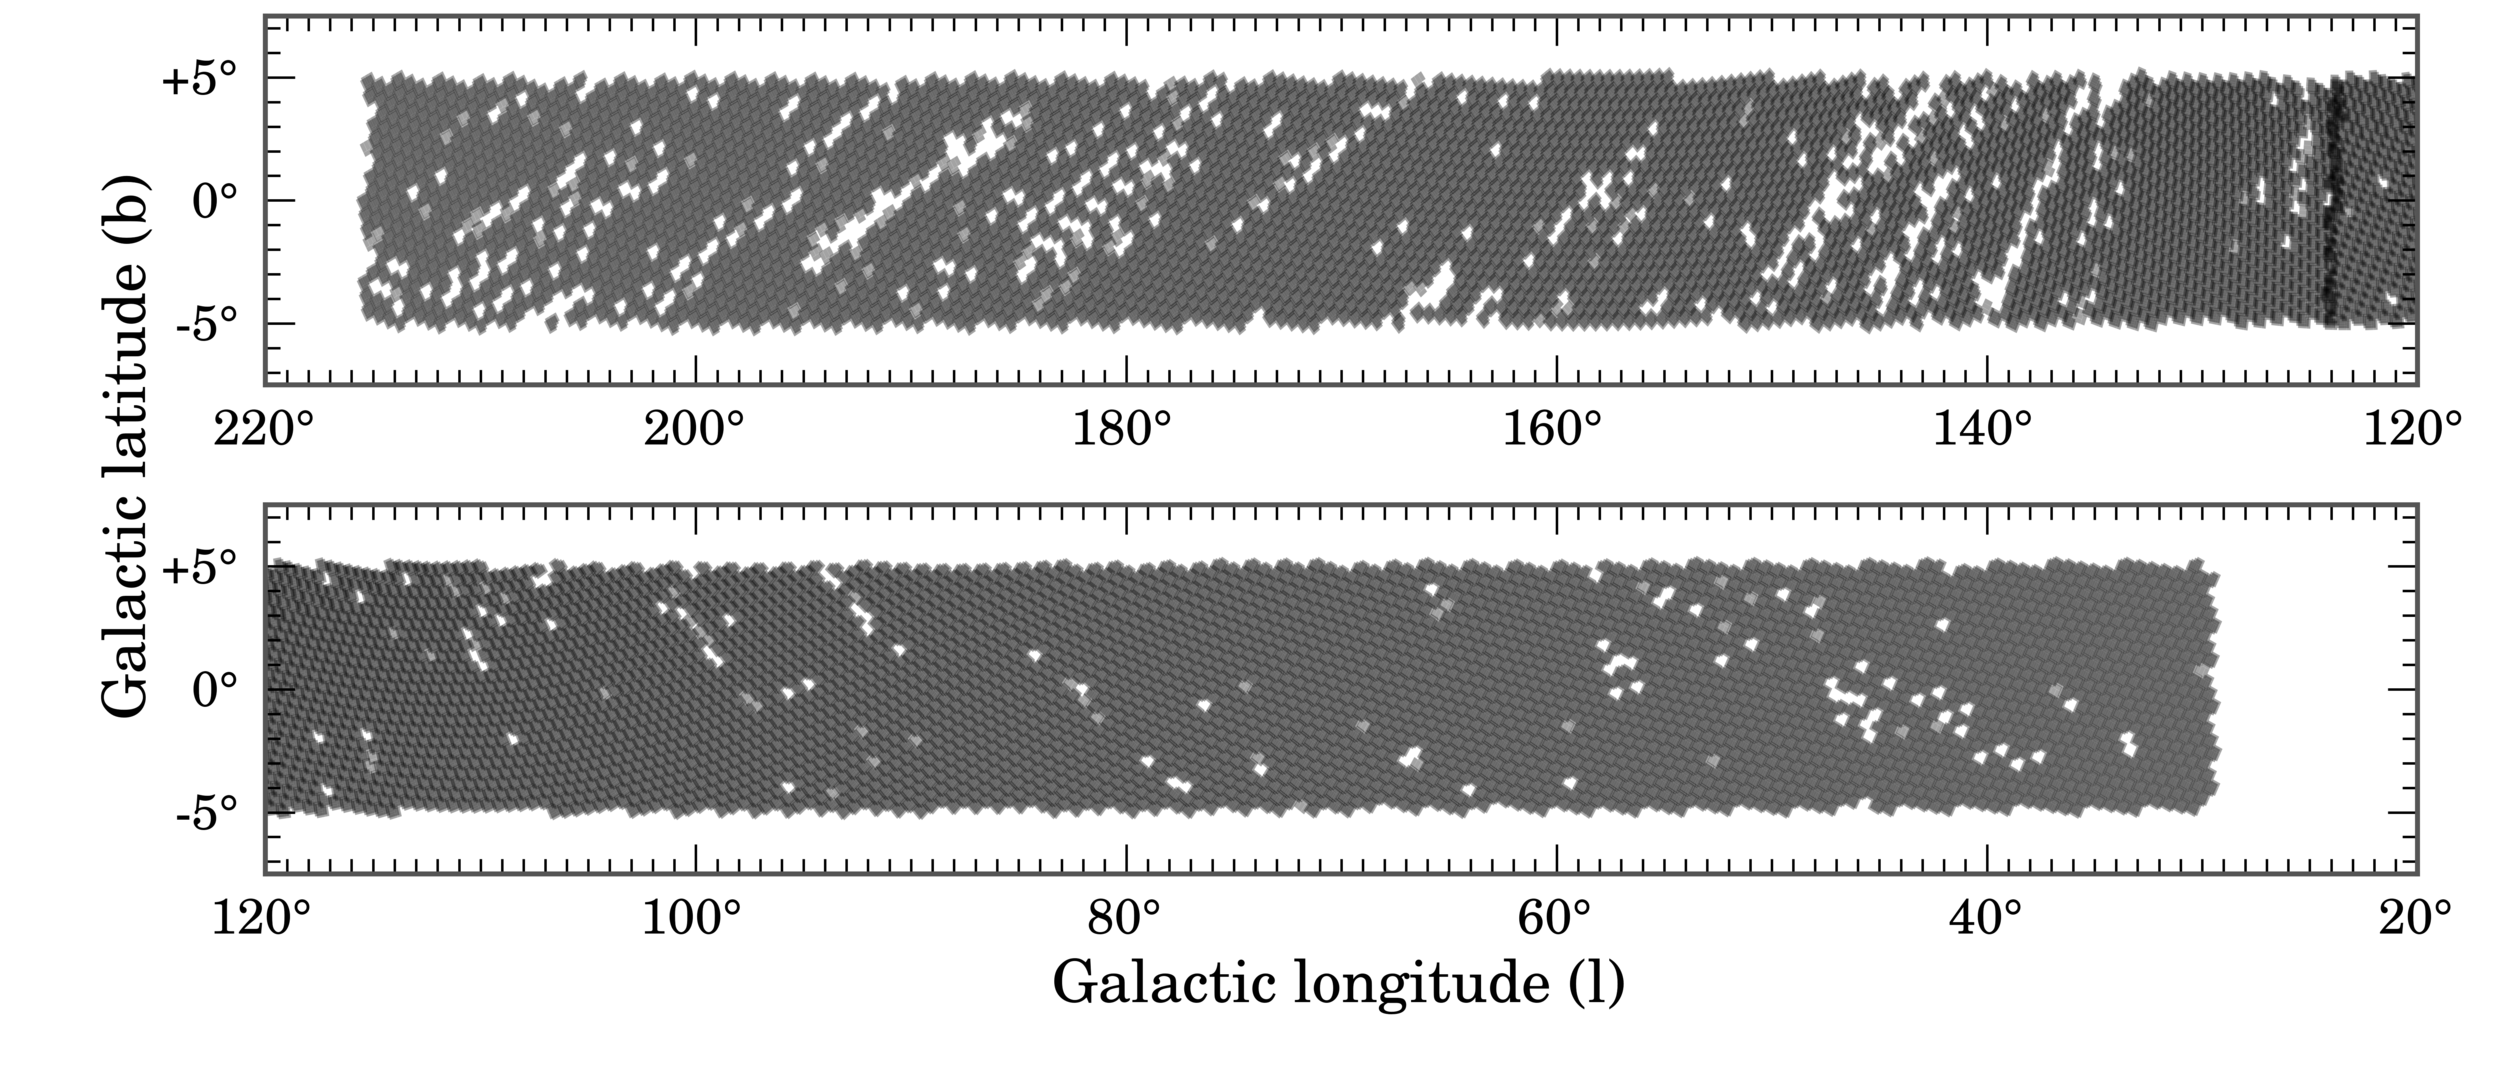
\includegraphics[width=1\linewidth]{./plots/footprint/footprint_small.png}
        \caption{Survey area showing the footprints
        of all the quality-approved IPHAS fields
        which have been included in this data release.
        The area covered by each field has been coloured black
        with a semi-transparent opacity of 20\%,
        such that regions where fields overlap are darker.
        The IPHAS strategy is to observe each field twice
        with a small offset,
        and hence the vast majority of the area 
        is covered twice (dominant grey colour).
        There are small overlaps between all the neighbouring fields
        which can be seen as a honeycomb pattern
        of dark grey lines across the survey area.
        Regions with incomplete data are apparent as white gaps (no data) 
        or in light grey (denoting that only one offset is missing).
        The dark vertical strip near $l \sim$125\deg
        is an arbitrary consequence of the tiling pattern,
        which was populated starting from 0h in right ascension.}
        \label{fig:footprint}
\end{figure*}

Fig.~\ref{fig:footprint} shows the footprin
of the quality-approved observations included in this work. 
The fields which remain missing 
-- covering 8\% of the survey area --
are predominantly located towards the Galactic anti-centre 
at $l > 120^o$.
Fields at these longitudes are mainly accessed from La Palma 
in the months of November-December,
which is when the La Palma weather and seeing conditions are often poor
forcing many (unsuccessful) repeat observations.
To enable the survey to be brought to completion, 
a decision was made recently to limit repeats in this area 
to individual fields requiring replacement,
i.e. fresh observations in all 3 filters may only be obtained 
at one of the two offset positions.  
The catalogue is structured such that it is clear 
where a contemporaneous observation of both halves of a field pair
is available.


\section{Data reduction and quality control}
\label{sec:reduction}

\subsection{Initial pipeline processing}

All raw IPHAS data were transferred
to the Cambridge Astronomical Survey Unit (CASU) 
for initial processing and archival.
The procedures used by CASU were originally devised
for the INT Wide Field imaging Survey \citep[WFS;][]{McMahon2001,Irwin2005},
which was a 200 deg$^2$ survey programme carried out 
between 1998 and 2003 after the WFC was commissioned.
Because IPHAS uses the same telescope and camera combination,
we have been able to benefit from the existing WFS pipeline.
A detailed description of the processing steps 
is found in \citet{Irwin2001}.
Its application to IPHAS has previously been described
by \citet{Drew2005} and \citet{Gonzalez-Solares2008},
and much of the source code is available 
on line\footnote{http://casu.ast.cam.ac.uk/surveys-projects/software-release}. 
In brief, the pipeline takes care of bias subtraction,
linearity correction, flat-fielding,
gain correction and de-fringing.

The reduced images are then stored in multi-extension FITS files
with a primary header describing the characteristics
(position, filter, exposure time, etc.) 
and four image extensions 
corresponding to each of the four CCDs.
Source detection and characterisation is then carried out 
using the \textsc{imcore} tool \citep{Irwin1985,Irwin1997}.
The flux of each source is measured using both
the peak pixel height
(i.e. a square 0.33$\arcsec\times$0.33\arcsec\ aperture)
and a series of circular apertures of increasing diameter 
(1.2\arcsec, 2.3\arcsec, 3.3\arcsec, 4.6\arcsec\ and 6.6\arcsec).

The local background levels are estimated 
by computing the sigma-clipped median
flux in a grid of 64$\times$64 pixels (21\arcsec$\times$21\arcsec)
across the image,
which is then interpolated to obtain an estimate 
of the background level at each pixel.
These sky levels are subtracted from the aperture photometry and
-- when required --
a deblending routine is applied to remove
the contamination from any nearby sources.
This approach works very well 
across the vast majority of the survey area.  Nevertheless,
the Galactic Plane contains crowded regions 
with large numbers of overlapping sources
or rapidly spatially-varying nebulosity,
where aperture photometry will be compromised by frequent blending
or poor background subtraction.
In \S\ref{sec:catalogue} we will explain how affected sources are 
flagged. 
%we will explain that objects affected in this way 
%are flagged in the catalogue using the \emph{deblend} warning flag.

Finally, an astrometric solution is determined
based on the Two-Micron All Sky Survey (2MASS) point source catalogue \citep{Skrutskie2006},
which itself is calibrated 
in the International Celestial Reference System (ICRS).
A provisional photometric calibration is also provided 
based on the average zeropoint
determined from sets of standard stars observed within the same night.
Sources are classified morphologically
-- stellar, extended or noise --
based on the curve-of-growth determined
from measuring the source intensity in a series of growing apertures.
Finally, the resulting source detection tables are also stored 
in multi-extension FITS files.

At the time of preparing DR2,
the CASU pipeline had processed
74\,195 IPHAS exposures 
in which a total of 1.9~billion \emph{candidate sources} were detected 
at the sensitive default detection level of 1.25\,$\sigma$.
This total inevitably includes spurious detections, artefacts and
duplicate detections,
in \S\ref{sec:catalogue} we will explain
how these have been removed or flagged in the final catalogue.
The pipelined data set -- comprising 2.5~terabyte of FITS files --
was then transferred to the University of Hertfordshire
for the purpose of transforming the raw
detection tables into a reliable source catalogue which is 
(i) quality-controlled,
(ii) homogeneously calibrated, and 
(iii) contains user-friendly columns and warning flags.
It is these post-processing steps which are explained next.


\subsection{Quality control}
\label{sec:qc}

Observing time for IPHAS was obtained
on a semester-by-semester basis
through the open time allocation committees 
of the Isaac Newton Group of telescopes,
which are invariably over-subscribed.
For this reason, we attempted to utilise 
\emph{all} the nights allocated to IPHAS,
even those which were partially or entirely non-photometric
or otherwise affected by technical problems 
(e.g. electronic noise or telescope tracking problems).
Any unsuitable data that were taken as a result
of this strategy have subsequently been flagged and removed
using seven quality criteria,
which ensure a reliable and homogeneous level of quality
across the data release:

\begin{figure}
    \begin{minipage}[b]{\linewidth}
        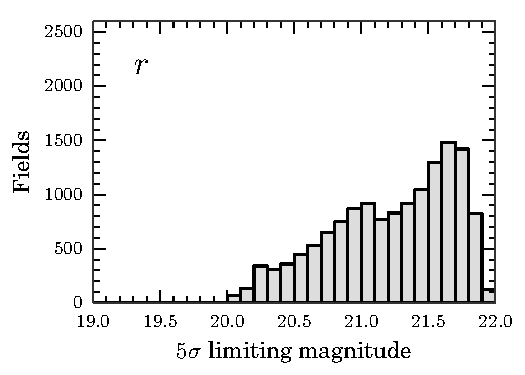
\includegraphics[width=\textwidth]{./plots/depth_r.pdf} 
    \end{minipage}
    \begin{minipage}[b]{\linewidth}
        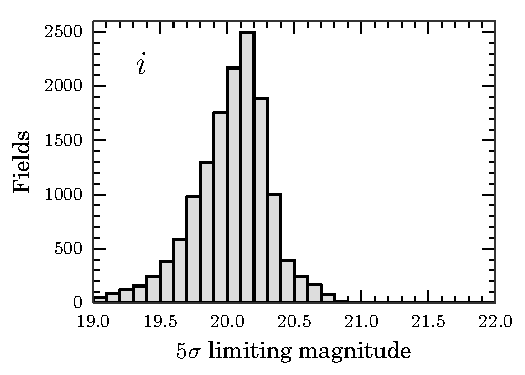
\includegraphics[width=\textwidth]{./plots/depth_i.pdf} 
    \end{minipage}
    \begin{minipage}[b]{\linewidth}
        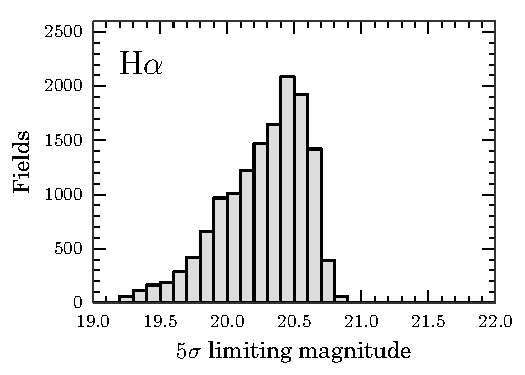
\includegraphics[width=\textwidth]{./plots/depth_h.pdf} 
    \end{minipage}
    \caption{Distribution of the 5$\sigma$ limiting magnitude
             across all quality-approved survey fields
             for $r$ (top), $i$ (middle) and \ha\ (bottom).
             Fields with a limiting magnitude brighter than
             20th ($r$) or 19th (\ha, $i$) were rejected
             from the data release.
             The $r$-band depth is most sensitive 
             to the presence of the moon above the horizon: 
             this is the reason for the wide, bi-modal character
             of its distribution.}
    \label{fig:depth}
\end{figure}

(1) \emph{Depth.} 
We discarded any exposures for which the $5\sigma$ limiting magnitude 
was worse than 20th magnitude in the $r$-band
or worse than 19th in $i$ or \ha. 
Such data were typically obtained during poor weather or full moon.
Most observations were significantly better than these limits.
Fig.~\ref{fig:depth} presents the distribution of limiting magnitudes
for all quality-approved fields,
showing mean depths of 
$21.2\pm0.5$ ($r$), $20.0\pm0.3$ ($i$) and $20.3\pm0.3$ (\ha).
The depth achieved depended 
most strongly on the presence of the moon,
which was above the horizon during 62\% 
of the observations.  The great range in sky brightness this
produced is the reason for the wide and bi-modal shape
of the $r$-band limiting magnitude distribution 
(top panel in Fig.~\ref{fig:depth}).
In contrast, the depths attained in $i$ and \ha\ 
are less sensitive to moonlight, leading to
narrower magnitude limit distributions
(middle and bottom panels in Fig.~\ref{fig:depth}).

(2) \emph{Ellipticity.} 
The ellipticity of a point source,
defined as $e = 1 - b / a$ 
with $b$ the semi-minor and $a$ the semi-major axis,
is a morphological measure of the elongation of the point spread function (PSF).
It is expected to be zero (circular) across the field 
in a perfect imaging system,
but it is slightly non-zero in any real telescope data 
due to optical distortions and tracking errors.
Indeed, it is worth noting
that IPHAS data have been collected
from unguided exposures that rely entirely
on the INT's tracking capability.
The mean ellipticity measured
in the data is $0.09\pm0.04$.
There have been sporadic episodes with higher ellipticities
due to mechanical glitches in the telescope tracking system.
To exclude these, we rejected exposures in which the mean ellipticity
across the detector exceeded $e > 0.3$.
We have also found that, as this threshold is breached,
the photometric measurements delivered by the pipeline become degraded.

(3) \emph{Seeing.} 
The original survey goal was to obtain data 
at a resolution better than 1.7~arcsec,
as evaluated by measuring the average PSF Full Width at Half Maximum (FWHM)
across an image,
which is a proxy for the combined effect of atmospheric and dome seeing.
This target is currently attained across 86\% of the footprint,
in particular at lower Galactic longitudes,
e.g. 92\% of the fields at $l<120^\circ$ are better than 1.7~arcsec.
To slightly increase the sky area offered by this data release,
we have decided to include data obtained under seeing of up to 2.5 arcsec.
Fig.~\ref{fig:seeing} presents the distribution
of the PSF FWHM for the approved fields in the release.
In the $r$-band, 90\% of the data is better than 1.5~arcsec,
50\% is better than 1.1~arcsec,
and 10\% is better than 0.8~arcsec.
In \S\ref{sec:catalogue} we will explain
that the photometry compiled in the source catalogue
is normally derived from the field with the
best-available seeing for a given object,
and that the PSF FWHM measurement
is included as a column in the catalogue.

\begin{figure}
    \begin{minipage}[b]{\linewidth}
        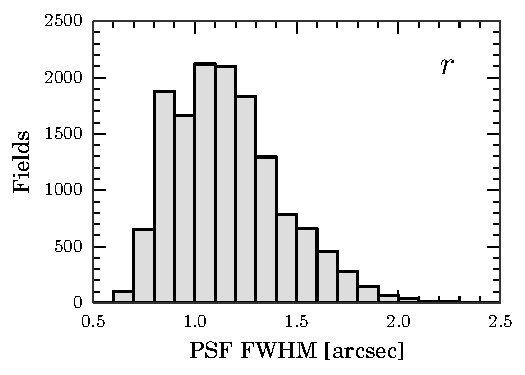
\includegraphics[width=\textwidth]{figures/seeing/seeing_r.pdf} 
    \end{minipage}
    \begin{minipage}[b]{\linewidth}
        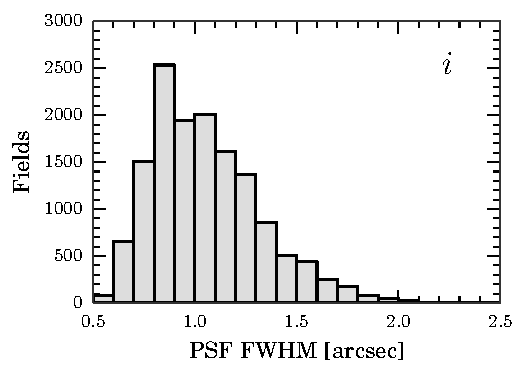
\includegraphics[width=\textwidth]{figures/seeing/seeing_i.pdf} 
    \end{minipage}
    \begin{minipage}[b]{\linewidth}
        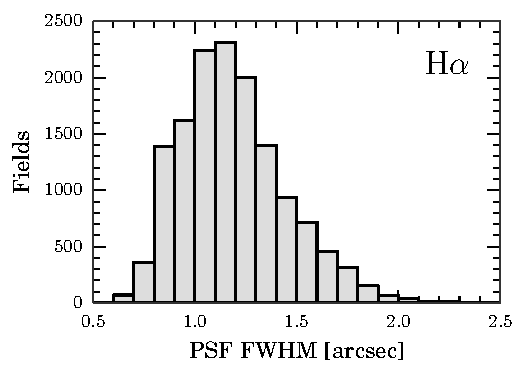
\includegraphics[width=\textwidth]{figures/seeing/seeing_ha.pdf} 
    \end{minipage}
    \caption{Distribution of the PSF FWHM
             for all the quality-approved fields
             included in the release,
             measured in $r$ (top), $i$ (middle) and \ha\ (bottom).
             The PSF FWHM measures the effective image resolution
             that arises from the combination of atmospheric and dome seeing.}
    \label{fig:seeing}
\end{figure}


(4) \emph{Photometric repeatability.} 
The IPHAS field-pair observing strategy normally
ensures that every pointing is immediately followed 
by an offset pointing at a displacement
of $+$5~arcmin in Dec and $+$5~arcmin in RA.
This allows pairs of images to be checked 
for the presence of clouds or electronic noise.
To exploit this information,
the overlap regions of all field pairs were systematically cross-matched
to verify the consistency of the photometry
for stars observed in both pointings.
We rejected field pairs in which more than 2\% of the stars 
showed an inconsistent measurement at the level of 0.2 mag,
or more than 26\% were inconsistent at the level of 0.1 mag.
These limits were set empirically after inspecting
the images and photometry by eye.

(5) \emph{Source density mapping.}
Spatial maps showing the number density of the detected sources
down to 20th magnitude were created to verify the health
of the data and to check for unexpected artefacts.
In particular, we created density maps
which showed the number of \emph{unique} sources
obtained by cross-matching the detection tables of
all three bands with a maximum matching distance of 1~arcsec.
This was particularly effective for revealing
fields with an inaccurate astrometric solution in one of the bands,
which were subsequently corrected.

(6) \emph{Visual examination.}
Images, colour mosaics,
and the associated photometric colour/magnitude diagrams
were inspected by a team of 20 survey members, 
such that each image in the data release 
was looked at by at least three different pairs of eyes.
Images affected by clouds or extreme levels of scattered moonlight
were flagged, investigated,
and excluded from the release 
by placing them on a \emph{black-list}.

(7) \emph{Contemporaneous field data.} 
Finally, only exposures which are part of a sequence 
of three consecutive images of the same field
(\ha, $r$, $i$)
were considered for inclusion in the release. 
This ensures that the three bands for a given field
are observed contemporaneously --  
normally within 5 minutes of each other.
An exception was made for 9 fields where the three exposures 
could not be obtained within the same night
but for which the time gap between exposures did not exceed 48 hours.
We note that the source catalogue details the exact epoch
at the start of each exposure
(columns \emph{rMJD}, \emph{iMJD}, \emph{haMJD}).

All of the above criteria were satisfied by at least one observing attempt
for 14\,115 out of the 15\,270 fields (92\%).
In some cases more than one successful attempt to observe
a field was available due to stricter
quality criteria being applied in the initial years of the survey.
In such cases, only the attempt 
with the best seeing and depth has been selected
for inclusion in the catalogue, in order  
to deliver the most reliable measurement at a single epoch.

We note that some of the excluded data may nevertheless be useful
for e.g. time-domain studies of bright stars.
The images and detection tables of the discarded data are made
available through our website for this reason (www.iphas.org),
but will be ignored in the remainder of this work.

\section{Photometric calibration}
\label{sec:calibration}

Having obtained a quality-approved set of observations,
we now turn to the problem of placing the data
onto a uniform photometric scale.

\subsection{Provisional nightly calibration}

For the purpose of providing an initial calibration 
of the $r$ and $i$ broadband fluxes,
photometric standard fields were observed every night.
The standards were chosen from a list based on 
the \cite{Landolt1992} and Stetson (http://cadcwww.dao.nrc.ca/standards) 
objects.
Two or three standard fields were observed 
during the evening and morning twilight,
and at intervals of 2-3 hours throughout the night.
The CASU pipeline automatically identified the observed standards 
and used them to determine a sigma-clipped average zeropoint \textsc{magzpt}
for each night and filter,
such that the number counts $DN$ 
in the pipeline-corrected CCD frames
relate to a magnitude $m$ as:
\begin{equation}
\begin{split}
   m  = & \textsc{magzpt} - 2.5 \log_{10}( DN / \textsc{exptime} ) \\
 &  - \textsc{extinct}\cdot(\textsc{airmass}-1) - \textsc{apcor} - \textsc{percorr},
\label{eqn:mag}
\end{split}
\end{equation}
where \textsc{exptime} is the exposure time in seconds,
\textsc{extinct} is the atmospheric extinction coefficient 
(set in the pipeline at 0.09 for $r$ and 0.05 for $i$ as representative
averages for La Palma),
\textsc{airmass} is the normalised optical path length 
through the atmosphere and
\textsc{apcor} is a correction for the flux
lost outside of the aperture used.
Finally, \textsc{percorr} is a correction based on the difference
between the median dark sky for a CCD against the median for all the CCDs, 
and as such is an ancillary correction 
to account for sporadic gain variations. 
All these quantities correspond to header keywords in the 
multi-extension FITS files produced by the CASU pipeline.

The broadband zeropoints were determined such that the resulting magnitude system
refers to the spectral energy distribution (SED) of Vega 
as the zero colour object. 
Colour equations were used to transform between the IPHAS passbands 
and the Johnson-Cousins system 
of the published standard star photometry.
The entire procedure has been found to deliver zeropoints which 
are accurate at the level of 1-2\% 
in photometric conditions \citep{Gonzalez-Solares2011}.

Unlike the broadbands, 
standard-star photometry is not available in the literature 
for the H$\alpha$ passband
and hence there is no formally recognised flux scale 
for it.
We can specify here, however, 
that the integrated in-band energy flux for Vega 
in the IPHAS \ha\ filter 
is $1.52 \times 10^{-7}$ ergs\,cm$^{-2}$\,s$^{-1}$ 
at the top of the Earth's atmosphere,
which is the flux obtained by folding 
Vega's SED with the filter transmission curve 
(uncorrected for the atmosphere and detector quantum efficiency,
which would otherwise scale down the narrowband flux by 0.707).
This is 3.14 magnitudes less than the flux captured 
by the much broader $r$ band
which includes the \ha\ band.
Hence to assure zero colour relative to the broadbands,
we set the default zeropoint for the narrowband to be:
\begin{equation}
\textsc{magzpt}_{H\alpha} = \textsc{magzpt}_r - 3.14.
\label{eqn:zpha}
\end{equation}
Note that the above implies that the in-band flux corresponding to
zero magnitude is $1.56 \time 10^{-7}$ ergs\,cm$^{-2}$\,s$^{-1}$,
when the \ha\ magnitude for Vega is set by convention to 0.03.


\subsection{Uniform re-calibration}

Despite the best efforts made to obtain a nightly calibration,
large surveys naturally possess field-to-field variations
at the level of 0.1 mag
due to atmospheric changes during the night
and imperfections in the pipeline or the instrument
(e.g. the WFC is known to suffer from sporadic errors
in the timing of exposures).
Such variations need to be corrected for 
during a global re-calibration procedure.
Notable past examples include the global re-calibration 
of 2MASS \citep[][]{Nikolaev2000},
SDSS \citep[][]{Padmanabhan2008}
and the Panoramic Survey Telescope 
And Rapid Response System survey \citep[Pan-STARRS;][]{Schlafly2012},
which all achieved photometry 
that is globally consistent to within 0.01--0.02~mag.

Surveys which observe identical stars at different epochs
can use the repeat measurements to ensure a uniform calibration.
For example, 2MASS attained its global calibration
by observing six standard fields each hour, 
allowing zeropoint variations to be tracked 
over very short timescales \citep{Nikolaev2000}.
Alternatively, the SDSS and PanSTARRS surveys could benefit
from revisiting regions in their footprint to 
carry out a so-called \emph{ubercalibration}\footnote{`Ubercalibration'
refers to the name of the code used to re-calibrate SDSS photometry
using repeat observations. 
It is an anglicised version of the German word `\"uberkalibration',
which was reportedly chosen because the initial authors both
had German-sounding names \citep{Finkbeiner2010}.} procedure,
in which multiple measurements of stars at different epochs
are used to fit the calibration parameters
\citep[e.g.][]{Ivezic2007,Padmanabhan2008,Schlafly2012}.

Unfortunately these schemes cannot be applied
directly to IPHAS
for two reasons. 
First, the survey was carried out 
in competitively-allocated observing time on a
common-user telescope, 
rendering the 2MASS approach 
of observing standards at a very high frequency
prohibitively expensive (it does not help that 
standard fields 
are very scarce within the Galactic Plane).
Second, IPHAS is not specified as a variability survey, with
the consequence that stars are not normally observed at more 
than one epoch,
unless they happen to fall within a narrow overlap region 
between two neighbouring field pairs.

Although the IPHAS data do contain a significant number of 
such inter-field repeat measurements,
we have found the information contained
in these regions to be insufficient
to constrain the calibration parameters.
This is because photometry at the extreme edges of the WFC
-- where neighbouring fields overlap -- 
is prone to systematics at the level of 1--2\%.
The cause of these errors is thought to include 
the use of twilight sky flats in the pipeline,
which are known to be imperfect for calibrating stellar photometry 
due to stray light and vignetting \citep[e.g.][]{Manfroid1995}.
Moreover, the illumination correction in the overlap regions
is more affected by a radial geometric distortion in the WFC,
which causes the pixel scale to increase as the edges 
are approached \citep{Gonzalez-Solares2011}.
Although these systematics are reasonably small within a single field,
they can combine, during the global calibration routine, to cause artificial zeropoint gradients 
across the survey unless controlled by other external constraints.

For these reasons, we have decided not to depend
on an ubercalibration-type scheme alone,
and have opted to involve an external reference survey
-- where available --
to bring the majority of our data onto a uniform calibration.

\subsubsection{Correcting zeropoints using APASS}

We have been able to benefit from the
AAVSO Photometric All-Sky Survey
(APASS; http://www.aavso.org/apass)
to bring most of the survey 
onto a uniform scale.
Since 2009,
APASS has been using two 20~cm-astrographs
to survey the entire sky down to $\sim$17th magnitude
in five filters which include Sloan $r$ and $i$ \citep{Henden2012}.
The most recent catalogue available 
at the time of preparing this work was APASS DR7,
which provides a good coverage across $\sim$half
of the IPHAS footprint.
The overlap regions are shown in Fig.~\ref{fig:apass_r}.
The photometric accuracy of APASS is currently estimated 
to be at the level of 3\% (Henden, private communication),
which is significantly better 
than the original nightly calibrations of IPHAS
which are accurate to $\sim$10\% (Tab.~\ref{tbl:offsets_before}).
APASS achieves its uniform accuracy 
by measuring each star at least two times in photometric conditions,
along with ample standard fields,
benefiting from the large 3-by-3 degrees field of view of its detectors.

With the aim of bringing IPHAS to a similar accuracy of 3\%,
we used the APASS catalogue to identify and adjust the calibration of all IPHAS fields 
which showed a magnitude offset larger than 3\% against APASS.  Experience of re-running
the calibration and testing the results showed us that it was inadvisable to more
finely tune the match for IPHAS data obtained in what were generally the most photometric
nights.  To this end,
the $r$- and $i$-band detection tables of each IPHAS field
were cross-matched against the APASS DR7 catalogue 
using a maximum matching distance of 1~arcsec.
The magnitude range was limited to
$13<r_{\rm APASS}<16.5$ and $12.5<i_{\rm APASS}<16.0$
in order to avoid sources 
brighter than the IPHAS saturation limit on one hand, 
and to avoid sources near the faint detection limit of APASS 
on the other.

The resulting set of $\sim$220\,000 cross-matched stars were then used 
to derive APASS-to-IPHAS magnitude transformations
using a linear least-squares fitting routine, 
which iteratively removed $3\sigma$-outliers to improve the fit.
The solution converged to:
\begin{align} 
r_{\rm IPHAS} = r_{\rm APASS} - 0.121 + 0.032(r-i)_{\rm APASS} \label{eqn:apass_r} \\
i_{\rm IPHAS} = i_{\rm APASS} - 0.364 + 0.006(r-i)_{\rm APASS} \label{eqn:apass_i}
\end{align}
The root mean square (rms) residuals of these transformations 
are 0.041 and 0.051, respectively.
The small colour terms in the equations
indicate that the IPHAS and APASS broadband filters 
are very similar.
The transformations include a large fixed offset,
but this is simply due to the fact that 
APASS magnitudes are given in the AB system
and IPHAS uses Vega-based magnitudes.
Separate transformations were derived for sight-lines 
with varying extinction properties to investigate the robustness
of the transformations with respect to different reddening regimes.
The variations at these different
sight-lines were found to be insignificant.
This is not surprising because heavily-reddened objects 
are naturally scarce at $r<16$.

Having transformed APASS magnitudes into the IPHAS system,
we then computed the median magnitude offset 
for each field which contained at least 30 cross-matched stars.
This was achieved for 48\% of our fields (shown in Figs.~\ref{fig:apass_r} and \ref{fig:apass_i}).
The mean offset was found to be
$0.014\pm0.104$~mag in $r$ and $0.007\pm0.108$~mag in $i$
(Table~\ref{tbl:offsets_before}).
A total of 4596 fields showed a median offset
exceeding $\pm$0.03~mag in either $r$ or $i$.

We then applied the most important step in our calibration scheme,
which is to adjust the provisional zeropoints of these 4596 aberrant fields
such that their offset is brought to zero.
This allowed the mean IPHAS-to-APASS offset 
to be brought down to $0.000\pm0.011$~mag in both $r$ and $i$
(Table~\ref{tbl:offsets_after}).
The procedure of fitting magnitude transformations and
correcting the IPHAS zeropoints was repeated a few times to ensure 
convergence, which was essentially reached after the first iteration.

\begin{figure*}
    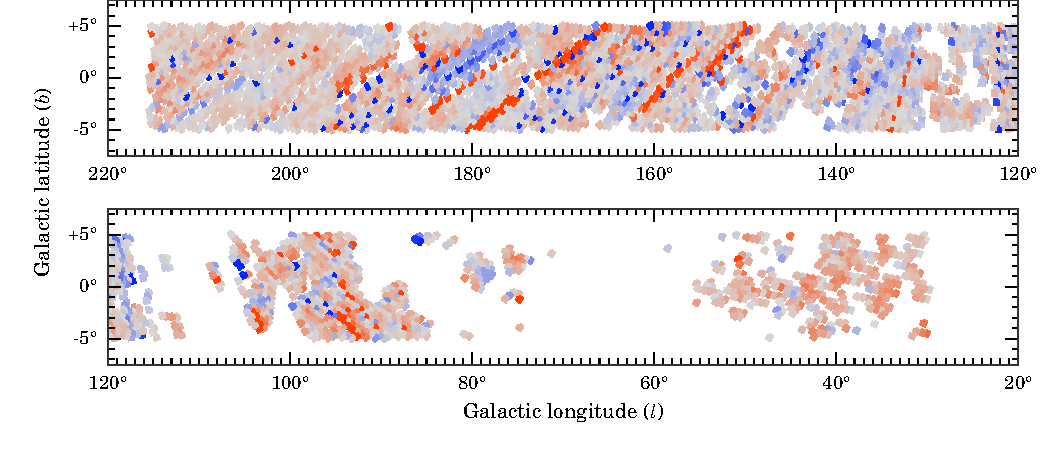
\includegraphics[width=\textwidth]{plots/calibration/APASS-IPHAS-DR2_rshift.pdf} 
    
\includegraphics[width=\textwidth]{plots/calibration/colourbar_apass_r.pdf} 
    \caption{Median magnitude offset in the $r$ band between IPHAS and APASS,
             plotted on a field-by-field basis
             prior to the re-calibration procedure.
             Each square represents the footprint of an IPHAS field
             which contains at least 30 stars with a counterpart
             in the APASS DR7 catalogue.
             The colours denote the median
             IPHAS-APASS magnitude offset in each field,
             which was computed after applying the APASS-to-IPHAS
             transformation to the APASS magnitudes (Eqn.~\ref{eqn:apass_r}).
             For clarity, we do not show the fields at the offset positions.}
        \label{fig:apass_r}
    \vspace{1cm}
    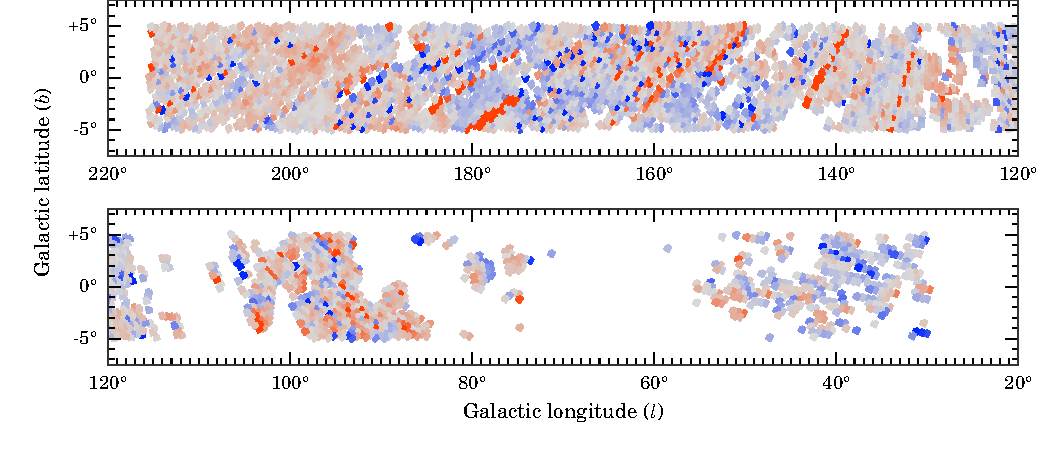
\includegraphics[width=\textwidth]{plots/calibration/APASS-IPHAS-DR2_ishift.pdf} 
    
\includegraphics[width=\textwidth]{plots/calibration/colourbar_apass_i.pdf} 
    \caption{Same as Fig.~\ref{fig:apass_r} for the $i$-band.}
    \label{fig:apass_i}
\end{figure*}

\begin{figure*}
    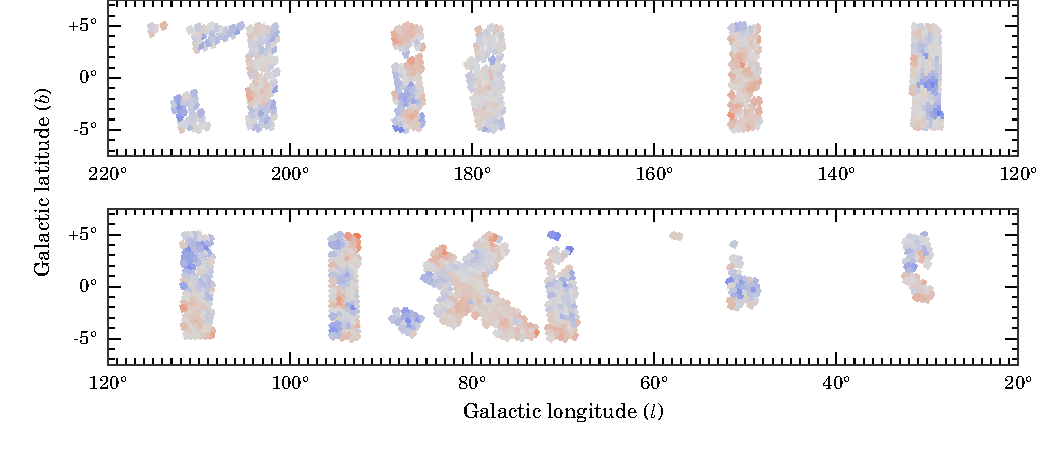
\includegraphics[width=\textwidth]{plots/calibration/SDSS-IPHAS_rshift.pdf}
    
\includegraphics[width=\textwidth]{plots/calibration/colourbar_sdss_r.pdf} 
    \caption{Median magnitude offset between IPHAS and SDSS in the $r$ band
             \emph{after} the re-calibration procedure was applied.
             Each square represents the footprint of an IPHAS field
             which contains at least 30 stars
             with a counterpart in the SDSS DR9 catalogue.
             The colours denote the median IPHAS-SDSS magnitude offset
             in each field,
             which was computed after applying the SDSS-to-IPHAS
             transformation to the SDSS magnitudes (Eqn.~\ref{eqn:sdss_r}).}
    \label{fig:sdss_r}
    \vspace{1cm}
    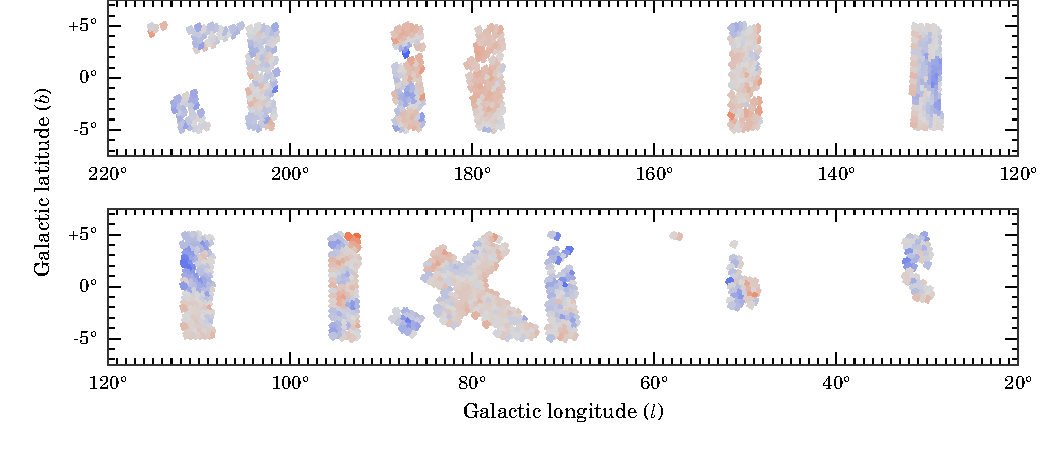
\includegraphics[width=\textwidth]{plots/calibration/SDSS-IPHAS_ishift.pdf}
    
\includegraphics[width=\textwidth]{plots/calibration/colourbar_sdss_i.pdf} 
    \caption{Same as Fig.~\ref{fig:sdss_r} for the $i$-band.}
    \label{fig:sdss_i}
\end{figure*}

\begin{table}
    \caption{Mean magnitude offsets for objects
             cross-matched between IPHAS and APASS/SDSS
             \emph{before} the uniform re-calibration was carried out.
             Transformations were applied
             to the APASS and SDSS magnitudes to bring them into the
             Vega-based IPHAS system prior to computing
             these statistics (see text).
             }
    \label{tbl:offsets_before}
    \begin{center}
        \begin{tabular}{lcc}
            \toprule
            {\bf Before re-calibration} & Mean & $\sigma$  \\
            \midrule
            $r$ (IPHAS - APASS) & +0.014 & 0.104 \\
            $i$ (IPHAS - APASS) & +0.007 & 0.108 \\
            $r$ (IPHAS - SDSS) & +0.016 & 0.088 \\
            $i$ (IPHAS - SDSS) & +0.010 & 0.089 \\
            \bottomrule
       \end{tabular}
       \caption{Same as Table~\ref{tbl:offsets_before}
                but computed \emph{after} the uniform re-calibration
                 was carried out.}
        \label{tbl:offsets_after}
            \begin{tabular}{lcc}
                \toprule
                {\bf After re-calibration} & Mean & $\sigma$ \\
                \midrule
                $r$ (IPHAS - APASS) & +0.000 & 0.011\\
                $i$ (IPHAS - APASS) & +0.000 & 0.011 \\
                $r$ (IPHAS - SDSS)  & -0.001 & 0.029\\
                $i$ (IPHAS - SDSS) & -0.002 & 0.032 \\
                \bottomrule
            \end{tabular}
        \end{center}
\end{table}

\subsubsection{Adjusting fields not covered by APASS}

At the time of writing, the APASS catalogue did not provide 
sufficient coverage for 7359 of our fields.
Fortunately, these fields are located mainly 
at low Galactic longitudes (cf. Figs.~\ref{fig:apass_r} and \ref{fig:apass_i}),
which were typically observed during the summer months
when photometric conditions are more prevalent at the telescope.
These remaining fields have nevertheless 
been brought onto the same uniform scale 
by employing an ubercalibration-style scheme,
which minimises the magnitude offsets between stars
located in the overlap regions between neighbouring fields.

An algorithm for achieving this minimisation
has previously been described by~\citet{Glazebrook1994}.
In brief, there are two fundamental quantities to be
minimised between each pair of overlapping exposures, 
denoted by the indices $i$ and $j$. 
Firstly, the mean magnitude difference between stars in the overlap
region $\Delta_{ij}=\langle m_i-m_j\rangle=-\Delta_{ji}$ is a local
constraint. 
Secondly, to ensure the solution does not stray far 
from the existing calibration, 
the difference in zeropoints 
$\Delta\mathrm{ZP}_{ij}=-\Delta\mathrm{ZP}_{ji}$ 
between each pair of exposures must also be minimised.

Minimisation of these two quantities is a linear least squares problem 
because the magnitude $m$ depends linearly on the ZP (Eqn.~\ref{eqn:mag}).
Hence we can find the ZP shift to be applied to each field 
by minimising the sum:
\begin{equation}
   S = \sum_{i=1}^N \sum_{j=1}^N w_{ij} \theta_{ij} (\Delta_{ij} + a_i - a_j)^2,
   \label{eqn:chi2}
\end{equation}
where $i$ denotes an exposure, 
$j$ an overlapping exposure, 
$N$ the number of exposures,
$a_i$ the ZP to solve for 
and $a_j$ the ZP of an overlapping field ($\Delta\mathrm{ZP}_{ij}=a_i-a_j$). 
$w_{ij}$ are weights set to the inverse square of the uncertainty in $\Delta_{ij}$,
and $\theta_{ij}$ is an overlap function 
equal to either 1 if exposures $i$ and $j$ overlap or 0 otherwise. 
Solving for $a_i$ is equivalent to solving $\partial
S/\partial a_i=0$, which gives the matrix equation:
\begin{equation}
   \sum_{j=1}^N A_{ij} a_j = b_j,
   \label{eqn:matrix}
\end{equation}
where 
\begin{eqnarray}
   A_{ij} &=& \delta_{ij} \sum_{k=1}^N w_{jk}\theta_{jk} - w_{ij} \theta_{ij},\label{eqn:aij}\\
   b_i &=& \sum_{j=1}^N w_{ij} \theta_{ij}\Delta_{ji} = -\sum_{j=1}^N w_{ij} \theta_{ij}\Delta_{ij}.\label{eqn:bi}
\end{eqnarray}

We enforce a strong external constraint
on the solution by keeping the zeropoint fixed 
for the 6\,756 fields which have already been compared
and calibrated against APASS.
We hereafter refer to these fields as \emph{anchors}.
It is asserted that the zeropoints $a_i$ of the anchor fields 
are known and not solved for.  However they do appear in the vector 
$b_j$ as constraints.  In addition to the APASS-based anchors, 
we selected 3\,273 additional anchor fields by hand
to provide additional constraints in regions not covered by APASS.
These extra anchors were deemed to have reliable zeropoints 
based on 
(i) the information contained in the observing logs,
(ii) the stability of the standard star zeropoints during the night, and
(iii) photometricity statistics provided by the Carlsberg Meridian Telescope,
which is located $\sim$500~m from the INT.

We then solved Eqn.~\ref{eqn:matrix} for the $r$ and $i$ bands
separately using the least-squares routine 
in Python's {\sc scipy.sparse} module for sparse matrix algebra.
This provided us with corrected zeropoints for the remaining fields,
which were shifted on average by $+0.02\pm0.11$ in $r$ 
and $+0.01\pm0.12$ in $i$ compared to their provisional calibration.
The outcome is validated in the next section.

We then turned to the uniform calibration of the \ha\ data.
It is not possible to re-calibrate the narrowband 
in the same way as the broadbands,
because the APASS survey does not offer \ha\ photometry.
We can reasonably assume however,
that the corrections required for $r$ and \ha\ are identical,
much of the time, because the IPHAS data-taking pattern ensured 
that a field's \ha\ and $r$-band exposures
were taken consecutively -- 
separated only by the $\sim$30~s read-out time.
Hence, we have corrected the \ha\ zeropoints 
by re-using the zeropoint adjustments that were derived for the $r$ band
in the earlier steps.
An exception was made for 3\,101 fields
for which our quality-control routines revealed
zeropoint variations which exceeded 0.03~mag 
between consecutive fields,
suggesting strongly non-photometric conditions.
In these cases, the \ha\ zeropoints of these fields
were adjusted by solving Eqn.~\ref{eqn:matrix}
rather than linking them directly to the $r$-band shift.

\subsection{Testing the calibration against SDSS}

Having re-calibrated all fields to the expected APASS accuracy of 3\%,
we turned to a different survey, SDSS Data Release 9 \citep{Ahn2012},
to validate the results.
SDSS DR9 includes several strips at low
Galactic latitudes,
providing data across 18\% of the fields in our data release.
We cross-matched the IPHAS fields against the subset of
objects marked as reliable stars in the SDSS catalogue\footnote{
We used the CasJobs facility located at http://skyserver.sdss3.org/CasJobs
to obtain photometry from the SDSS {\sc photoprimary} table 
with criteria {\sc type = star}, {\sc clean = 1} and {\sc score $>$ 0.7}.}
cross-matching in much the same way as for APASS,
with the difference of selecting from the  fainter magnitude ranges of 
$15<r_{\rm SDSS}<18.0$ and $14.5<i_{\rm SDSS}<17.5$.
This provided us with a set of 1.2~million cross-matched stars.

Colour transformations were again obtained using a sigma-clipped linear least squares fit:
\begin{eqnarray}
r_{\rm IPHAS} = r_{\rm SDSS} - 0.093 - 0.044(r-i)_{\rm SDSS} \label{eqn:sdss_r} \\
i_{\rm IPHAS} = i_{\rm SDSS} - 0.318 - 0.095(r-i)_{\rm SDSS}. \label{eqn:sdss_i}
\end{eqnarray}
The rms residuals of these transformations are 0.045 and 0.073, respectively.
The equations are similar to the ones
previously determined for APASS,
although the colour terms are slightly larger.
The throughput curve of the SDSS $i$-band filter 
appears to be somewhat more sensitive at longer wavelengths
than both the IPHAS and APASS filters.

These global transformations were deemed adequate
for the purpose of validating our uniform calibration in a statistical sense.
Separate equations were derived towards different sight-lines
to investigate the effects of varying reddening regimes.
The colour term was found 
to show some variation towards lowly reddened areas,
where red objects at $(r-i) > 1$ are rare.
The vast majority of red objects in the global sample
are those in highly reddened areas however,
which agree well with the global transformations
and dominate the statistical appraisal of our calibration.

Having transformed SDSS magnitudes into the IPHAS system,
we then computed the median magnitude offset for each IPHAS field
which contained at least 30 objects with a cross-matched counterpart
in SDSS.  This was the case for 2\,602 fields.
The median offsets for each of these fields
are shown in Figs.~\ref{fig:sdss_r} and \ref{fig:sdss_i}.
Importantly, the mean offset and standard deviation found 
is $-0.001\pm0.029$~mag in $r$
and $-0.002\pm0.032$~mag in $i$ (Table~\ref{tbl:offsets_after}).
In comparison, offsets computed in the identical way
\emph{before} carrying out our re-calibration showed means
of $+0.016\pm0.088$~mag in $r$ and $+0.010\pm0.089$~mag in $i$ (Table~\ref{tbl:offsets_after}).
We conclude that our re-calibration procedure has
been successful in improving the
uniformity of the calibration by a factor three
and has achieved our aim of bringing the
accuracy down to the level of 0.03~mag (rms).

We warn that the SDSS comparison revealed a number of fields where the offsets
exceeded 0.05~mag (523 fields) or even 0.1~mag (18 fields).
This pattern of outliers is consistent with the tails of a Gaussian distribution
with $\sigma=0.03$.  Furthermore, it should not
be forgotten that both the SDSS and APASS calibrations are approximations to
perfection and will not be entirely free of anomalies.  Indeed as we worked, 
we noticed the occasional unsurprising examples of inconsistency between these 
two surveys.

\section{Source catalogue generation}
\label{sec:catalogue}

Having obtained a quality-checked 
and re-calibrated data set, 
we now turn to the problem
of transforming the observations 
into a user-friendly catalogue.
The aim is to present
the best-available information for each unique source
in a convenient format,
including flags to warn about quality issues 
such as source blending and saturation.
Compiling the catalogue involved four steps:
\begin{enumerate}
\item the single-band detection tables 
produced by the CASU pipeline 
were augmented with new columns
and warning flags;
\item the detection tables were merged into multi-band field catalogues;
\item the overlap regions of the field catalogues 
were cross-matched to flag duplicate measurements 
and identify the primary (best) detection 
of each unique source; and
\item these primary detections
were compiled into the final source catalogue.
\end{enumerate}
Each of these four steps are explained next.

\subsection{User-friendly columns and warning flags}

Enhancement of the detection tables by creating new columns
is the necessary first step because the tables generated by the CASU pipeline
refer e.g. to source positions in pixel coordinates, to photometric measures 
in number counts etc., rather than in directly useful astronomical terms.
To transform these data into user-friendly quantities,
we have largely adopted the units and naming conventions
which are in use at the 
WFCAM Science Archive \citep[WSA;][]{Hambly2008}
and the VISTA Science Archive \citep[VSA;][]{Cross2012}.
These archives curate the high-resolution near-infrared photometry from both
the UKIDSS Galactic Plane Survey \citep[GPS;][]{Lucas2008}
and the 
VISTA Variables in the Via Lactea survey \cite[VVV;][]{Minniti2010}.
There is a significant degree of overlap
between the footprints of UKIDSS/GPS and IPHAS,
and hence by adopting a similar catalogue format
we hope to facilitate scientific applications
which combine both data sets.

A detailed description of each column in our source catalogue
is given in Appendix~\ref{app:columns}.
In the remainder of this section we highlight the main features.

First, we note that each source is uniquely identified by an
IAU-style designation of the form ``IPHAS2\ JHHMMSS.ss+DDMMSS.s''
(cf. column \emph{name} in Appendix~\ref{app:columns}),
where ``IPHAS2'' refers to the present
data release and the remainder of the string
denotes the J2000 coordinates in sexagesimal format.
For convenience, the coordinates
are also included in decimal degrees
(columns \emph{ra} and \emph{dec})
and in Galactic coordinates
(columns \emph{l} and \emph{b}).
We have also included an internal object identifier string 
of the form ``\#run-\#ccd-\#detection''
(e.g. ``64738-3-6473''),
which documents the INT exposure number (\#run),
the CCD number (\#ccd),
and the row number in the CASU detection table (\#detection).
These columns are named \emph{rDetectionID},
\emph{iDetectionID}, \emph{haDetectionID}.

Photometry is provided based on the 2.3-arcsec diameter circular aperture
by default (columns \emph{r}, \emph{i}, \emph{ha}).
The choice of this aperture size as the default 
is based on a trade-off between concerns 
about small number statistics and centroiding errors
for small apertures on one hand,
and diminishing signal-to-noise ratios and source confusion
for large apertures on the other hand.
The user is not restricted to this choice, because
the catalogue also provides magnitudes
using three alternatives:
the peak pixel height 
(columns \emph{rPeakMag}, \emph{iPeakMag}, \emph{haPeakMag}),
the circular 1.2-arcsec-diameter aperture 
(\emph{rAperMag1}, \emph{iAperMag1},
 \emph{haAperMag1}) and
the 3.3-arcsec-diameter aperture 
(\emph{rAperMag3}, \emph{iAperMag3},
 \emph{haAperMag3}).

Each of these magnitude measurements have been
corrected for the flux lost outside of their respective apertures,
using a correction term which is inferred from the
mean shape of the PSF measured locally in the CCD frame.
In the case of a point source,
the four alternative magnitudes are expected
to be consistent with each other
within the photon noise uncertainty
(which is given in columns \emph{rErr}, \emph{rPeakMagErr},
\emph{rAperMag1Err}, \emph{rAperMag3Err}, etc).
When this is not the case,
it is likely that the source is either
an extended object for which the aperture correction is invalid,
or that the object has been incorrectly measured as a result of
source blending or a rapidly spatially-varying nebulous background.
In \S\ref{sec:qualitycriteria} we will explain that the consistency
of the different-aperture magnitude measurements
can be used as a criterion for selecting stellar objects
with reliable photometry from the catalogue.

The brightness of each object as a function of increasing
aperture size is also used by the CASU pipeline to provide
a discrete star/galaxy/noise classification flag
(\emph{rClass}, \emph{iClass}, \emph{haClass})
and a continuous stellarness-of-profile statistic
(\emph{rClassStat}, \emph{iClassStat}, \emph{haClassStat}).
For convenience, we have combined
these single-band morphological measures
into band-merged class probabilities and flags
using the merging scheme in use at the WSA\footnote{Explained at
http://surveys.roe.ac.uk/wsa/www/gloss\_m.html \#gpssource\_mergedclass
} (\emph{pStar}, \emph{pGalaxy}, \emph{pNoise},
\emph{mergedClass}, \emph{mergedClassStat}).


Information on the quality of each detection is included 
in a series of additional columns.
We draw attention to three useful flags
which warn about the likely presence of a systematic error:
\begin{enumerate}
\item The \emph{saturated} column is used to flag sources
for which the peak pixel height exceeds 55000 counts,
which is typically the case for stars brighter than 12-13th magnitude in
$r$.  Although the pipeline attempts to extrapolate the brightness of
saturated stars based on the shape of the PSF,
such extrapolation is prone to error,
and shoud be viewed as indicative rather than as precise measurement.
%and we do not recommend reliance on it.
\item The \emph{deblend} column is used to flag sources 
which partially overlap with a nearby neighbour.
Although the pipeline applies a deblending procedure
to such objects, the procedure is currently applied separately
in each band, and hence the $(r-i)$ and $(r-\ha)$ colours
may be inaccurate if the deblending proceeded differently in each band.
\item The \emph{brightNeighb} column is used to flag sources which are located
within a radius of 5 arcmin from an object brighter than $V=7$ 
according to the Bright Star Catalogue (BSC; Hoffleit et al. 1991), 
or within 10 arcmin if the neighbour is brighter than $V=4$.
These brightest stars are known to cause systematic errors
and spurious detections as a result of stray light 
and diffraction spikes.
\end{enumerate}
In addition to the above, we also created warning flags for internal bookkeeping.
For example, we flagged detections which fell in the strongly vignetted regions of the focal plane,
which were truncated by CCD edges,
or which were otherwise affected by bad pixels in the detector.
No such detections have had to be included in the catalogue, as 
alternative detections were available in essentially all these situations
thanks to the IPHAS field pair strategy. In turn, this has meant
that it has not proved necessary to include these internal warning flags
in the pubished source catalogue.

Finally, we note that basic information on the observing conditions
is included (\emph{fieldID}, \emph{fieldGrade}, \emph{night}, \emph{seeing}).
A table containing more detailed quality control information,
indexed by \emph{fieldID}, is made available on our website.

\subsection{Band-merging the detection tables}

The second step in compiling the source catalogue
is to merge the contemporaneous trios
of $r$, $i$, \ha\ detection tables
into multi-band field catalogues.
This required a position matching procedure 
to link sources between the three bands.
We used the \textsc{tmatchn} function 
of the \textsc{stilts} software for this purpose,
which allows rows from multiple tables to be matched \citep{Taylor2006}.
The result of the procedure is a band-merged catalogue
in which each row corresponds to a group of linked $r$, $i$, and \ha\ detections
which satisfy a maximum matching distance criterion in a pair-wise sense.
Sources for which no counterpart was identified
are retained in the catalogue as single-band detections.

We employed a maximum matching distance of 1~arcsec,
which was chosen, trading off completeness against reliability.
On the one hand, a matching distance larger than 1~arcsec 
was found to allow too many spurious and unrelated sources 
to be linked. 
On the other, a value smaller than 1~arcsec 
would pose problems for very faint sources 
with large centroiding errors, 
and would occasionally fail near CCD corners,
where the astrometric solution can 
show systematic errors which exceed 0.5~arcsec.
The position offsets between the $r$ detection and detections in $i$, and/or \ha\
have been included in the catalogue, giving the user the option to tighten them 
further if necessary
(columns \emph{iXi}, \emph{iEta}, \emph{haXi}, \emph{haEta}).
We note that UKIDSS/GPS adopted 
the same maximum matching distance of 1 arcsec
for similar reasons \citep{Hambly2008},
and warn that applications which require absolute
astrometry with sub-arcsecond accuracy must
use these catalogues with caution.

The resulting band-merged catalogues were found
to be reliable for the vast majority of fields.
We do warn that source blending and confusion is unavoidable
for faint objects in the most crowded regions of the Galactic Plane;
in \S\ref{sec:discussion} we will show
that 19\% of the sources in our catalogue
are flagged as blended objects (column \emph{deblend}),
and their band-merged data should be treated with care
because they may have fallen victim to source confusion
during the band-merging step.

\subsection{Selecting the primary detections}

We explained earlier that the survey contains repeat observations
of identical sources as a result of field offsetting and overlaps.
Amongst all sources in the magnitude range $13<r<19$,
we find that 65\% were detected twice and 25\% were detected three times or more.
Only 9\% were detected once.
%Unsurprisingly, their spatial distribution traces
%the inter-CCD gaps and footprint edges.

Since the principal aim of this data release is to provide 
reliable photometry at a single epoch,
we have focused on providing the magnitudes
and coordinates from the \emph{best-available} 
detection of each object -- 
hereafter referred to as the \emph{primary} detection.
Although overlapping fields could have been co-added 
to gain a small improvement in depth, 
we have decided against this for two reasons.
Firstly, combining the information from multiple epochs
would make the photometry of variable stars difficult to interpret.
Secondly, co-adding would cause the image quality to degrade towards the mean,
which is particularly a draw-back for crowded fields.

Anyone interested in the alternative detections of a source
-- hereafter called the \emph{secondary} detections --
can nevertheless obtain this information in two ways.
To begin with, whenever a secondary detection was collected 
within 10 minutes of the primary,
we have included the identifier and the default photometry
of that secondary detection
in the catalogue for convenience
(columns \emph{sourceID2}, \emph{fieldID2}, 
\emph{r2}, \emph{i2}, \emph{ha2},
\emph{rErr2}, \emph{iErr2}, \emph{haErr2}, \emph{errBits2}).
Such a secondary detection is available for 66\% of the sources brighter than $r<20$
due to the IPHAS field pair strategy.
In addition, the complete set of detection tables -- one for each exposure -- 
is made accessible on our website to allow other uses of the data.
%A user-friendly catalogue of secondary detections 
%has not been compiled at present 
%but may be part of a future data release.

%The primary detection is defined as the entry in the 
%set of band-merged field catalogues which provides 
%the most reliable information for a unique source.
Primary detections have been selected from all available detections using a so-called \emph{seaming} procedure,
which we adapted from the algorithm developed for the WSA\footnote{http://surveys.roe.ac.uk/wsa/dboverview.html\#merge}.
In brief, the first step is to identify all the duplicate detections
by cross-matching the overlap regions of all field catalogues,
again using a maximum matching distance of 1\arcsec.
The duplicate detections for each unique source are then ranked according to
(i) filter coverage, (ii) quality score (column \emph{errBits}),
and (iii) the average seeing of stars in the CCD frame rounded to 0.2~arcsec.
If this ranking scheme reveals multiple `winners' of seemingly identical quality,
then the one that was observed closest to the optical axis of the camera is chosen.


\subsection{Compiling the final source catalogue}

As the final step, the primary detections
selected above were compiled
into the 98-column source catalogue
that is described in Appendix~\ref{app:columns}
and is made available on our website and through Vizier.
The original unweeded list of sources naturally included 
a significant number of spurious entries
as a result of the very sensitive default detection settings
that are employed by the CASU pipeline.
To limit the size of the source catalogue,
we have decided to enforce three basic criteria
which must be met for a candidate source
to be included in the catalogue:
\begin{enumerate}
\item the source must have been detected at S/N$>5$ in at least
one of the bands, i.e. it is required that at least one of
\emph{rErr}, \emph{iErr} or \emph{haErr} is smaller
than 0.2 mag;
\item the shape of the source must not be an obvious
cosmic ray or noise artefact, i.e. we require
either \emph{pStar} or \emph{pGalaxy} to be
greater than 20\%;
\item the source must not have been detected in one of the strongly
vignetted corners of the detector, 
not have had any known bad pixels in the aperture,
and not have been on the edge of one of the CCDs,
i.e. we require the \emph{errBits} quality score
to be smaller than 64.
\end{enumerate}

A total of 219 million primary detections satisfied
the above criteria and have been included in the catalogue.
Amongst these, 158 million objects 
are detected in all three bands (72\%),
30 million are detected in two bands (14\%),
and 31 million entries are single-band detections (14\%).
Half of the single-band detections were made in the $i$-band.
This is because $i$ is least
affected by interstellar extinction and can occasionally pick up
highly-reddened objects which are otherwise lost in $r$ and \ha.

\section{Discussion}
\label{sec:discussion}

%Having explained how the catalogue was created,
We now offer an overview of the properties of the
catalogue by discussing  
(i) the recommended quality criteria,
(ii) the photometric uncertainties and repeatability,
and (iii) the source densities and the frequency of source blending.

\subsection{Recommended quality criteria}
\label{sec:qualitycriteria}

Like any other photometric survey,
the majority of the objects in our catalogue
are faint sources observed near the detection limits;
55\% of the entries in the catalogue
are fainter than $r > 20$.
%and 18\% are even fainter than $r > 21$.
The measurements of faint objects
are naturally prone to larger
random and systematic uncertainties:
for example, an inaccurately-subtracted background
will introduce a proportionally larger systematic error
for a faint object.
Most scientific applications will hence require a set of
quality criteria to be enforced for the purpose
of removing lower-quality objects.

The choice of quality criteria will always tension 
completeness against accuracy.
To aid users we have listed two sets of
recommended quality criteria 
in Tables~\ref{tab:reliable} and \ref{tab:veryreliable}.

Table~\ref{tab:reliable} specifies
a set of minimum quality criteria
which should benefit most applications
which desire reliable $(r-i)$ and $(r-\ha)$ colours
as well as completeness.
The listed criteria are designed to 
(i) remove low-S/N sources, 
(ii) remove saturated sources,
and (iii) remove objects for which the 2.3-arcsec diameter
aperture magnitude is inconsistent 
with its alternative 1.2-arcsec diameter measurement.
This last criterion is a proxy
for identifying objects which are affected
by poor background subtraction
or failed source deblending.
A total of 86 out of 219 million sources 
(39\%) satisfy all the criteria listed in Table~\ref{tab:reliable}
and are hereafter referred to as ``reliable''.
For convenience, the catalogue contains a boolean column
named \emph{reliable} that directly flags these objects.

\begin{table*}
\vspace{2cm}
\caption{Recommended minimum quality criteria 
for selecting objects with reliable colours 
from the IPHAS DR2 source catalogue. 
86~million entries in the catalogue (39\%)
satisfy all the criteria listed in this table.
For convenience, these have been flagged in the catalogue
using the column named \emph{reliable}.}
\begin{tabular}{p{8cm}lp{6cm}}
  \hline
  Quality criterion & Rows passed & Description \\
  \hline
  rErr\,$<$\,0.1 {\sc and} iErr\,$<$\,0.1 {\sc and} haErr\,$<$\,0.1 &
  109 million (50\%) &
  Require the photon noise to be less than 
  0.1 mag in all bands (i.e. S/N$>$10).
  This implicitly requires a detection in all three bands.  \\
  $r>13$ {\sc and} $i>12$ {\sc and} \ha\,$>12.5$ {\sc and not} \emph{saturated} &
  158 million (72\%) &
  The brightness must not exceed the nominal saturation limit
  and the peak pixel height must not exceed 55\,000 counts.
  Again, this implicitly requires a detection in all three bands.
  \\
  $|\mathrm{r}- \mathrm{rAperMag1}| 
  < 3\sqrt{\mathrm{rErr}^2 + \mathrm{rAperMag1Err}^2} 
  + 0.03$ &
  176 million (80\%) &
  Require the $r$ magnitude measured 
  in the default 2.3\arcsec\ diameter aperture
  to be consistent with the measurement 
  made in the smaller 1.2\arcsec\ aperture,
  albeit tolerating a 0.03 mag systematic error.
  This will reject sources for which the background
  subtraction or the deblending procedure
  was not performed reliably. \\
  $|\mathrm{i}- \mathrm{iAperMag1}| 
  < 3\sqrt{\mathrm{iErr}^2 + \mathrm{iAperMag1Err}^2} 
  + 0.03$ &
  183 million (84\%) &
  Same as above for $i$. \\
  $|\mathrm{ha}- \mathrm{haAperMag1}| < 
  3\sqrt{\mathrm{haErr}^2 + \mathrm{haAperMag1Err}^2} 
  + 0.03$ &
  158 million (72\%) &
  Same as above for \ha. \\
  \hline
  All of the above (flagged as {\bf\emph{reliable}}) &
  86 million (39\%) & \\
  \hline
\end{tabular}
\label{tab:reliable}

\vspace{2cm}
\caption{Additional quality criteria which are recommended
for applications which require very reliable colours
at the expense of completeness. 
For convenience, the sources which satisfy the criteria listed
in this table have been flagged in the catalogue
using the column named \emph{veryReliable}.}
\begin{tabular}{p{8cm}lp{6cm}}
  \hline
  Quality criterion & Rows passed & Description \\
  \hline
   reliable &
   86 million (39\%) &
   The object must satisfy the criteria listed in Table~\ref{tab:reliable}. \\
   
   pStar $>$ 0.9 &
   145 million (66\%) &
   % pStar > 0.89 is identical to mergedClass == -1
   The object must appear as a perfect point source,
   as inferred from comparing its PSF
   with the average PSF measured in the same CCD. \\
   
   {\sc not} \emph{deblend} &
   177 million (81\%) &
   The source must appear as a single, unconfused object. \\
   
   {\sc not} \emph{brightNeighb} &
   216 million (99\%) &
   There is no star brighter than $V < 4$ within 10 arcmin, 
   or brighter than $V < 7$ within 5 arcmin.
   Such very bright stars cause scattered light and diffraction spikes,
   which may add systematic errors to the photometry
   or even trigger spurious detections. \\  
  \hline
  
  All of the above (flagged as {\bf\emph{veryReliable}}) &
  59 million (27\%) & \\
  \hline
\end{tabular}

\label{tab:veryreliable}

\vspace{1cm}
\end{table*}

For applications which require
a higher standard of reliability at the expense of completeness,
a further set of additional quality criteria
are suggested in Table~\ref{tab:veryreliable}.
These criteria are designed to ensure that
(i) the object appeared as a perfect point source,
(ii) the object was not blended with a nearby neighbour,
and (iii) the object was not located near a very bright star.
59 million sources (27\%) satisfy
these stricter criteria 
and are hereafter referred to as ``very reliable''.
Again, the catalogue contains a boolean column
named \emph{veryReliable} which flags these objects.

Fig.~\ref{fig:magdist} compares the $r$-band magnitude
distributions for \emph{reliable}, \emph{veryReliable}
and unfiltered objects.
We find that 81\% of the sources 
are considered \emph{reliable}
and 54\% are \emph{veryReliable}
in the magnitude range $13 < r < 19$.
We will explain below that the
\emph{veryReliable} category is least complete
at low Galactic longitudes,
where source blending can affect
up to a quarter of the objects.
The \emph{veryReliable} flag should hence
only be used in applications in which 
completeness is not a concern.

\begin{figure}
    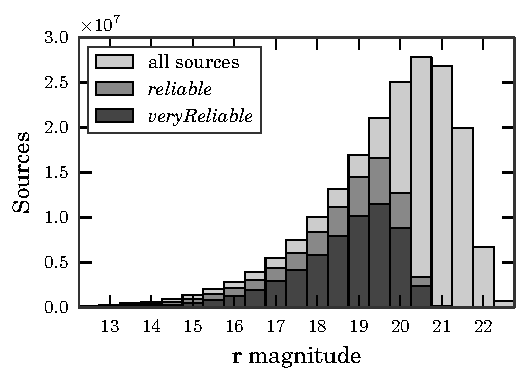
\includegraphics[width=0.5\textwidth]{./plots/magdist/magdist-r.pdf} 
    \caption{r-band magnitude distribution for all objects in the catalogue 
    (light grey), for objects flagged as \emph{reliable} 
    according to the criteria set out in Table~\ref{tab:reliable} (grey),
    and for objects flagged as \emph{veryReliable} 
    following Table~\ref{tab:veryreliable} (dark grey).
    The magnitude distributions for $i$ and \ha\
    look identical, apart from being shifted
    by about 1 and 0.5 mag towards brighter magnitudes,
    respectively.}
    \label{fig:magdist}
\end{figure}

It is easy to see how the quality criteria
may be adapted to be more tolerant.
For example, by raising the allowed photometric uncertainties
from 0.1~mag to 0.2~mag,
42 million candidate sources would be added to the 109 
million satisfying the tighter error bound.
Our choice to adopt 0.1~mag as the cut-off uncertainty
for the \emph{reliable} category is a pragmatic trade-off
which we found to suit many science applications,
but certainly not all. Users of the data are encouraged 
to revise the quality criteria according to their needs.

\subsection{Random and systematic uncertainties}

\begin{figure}
    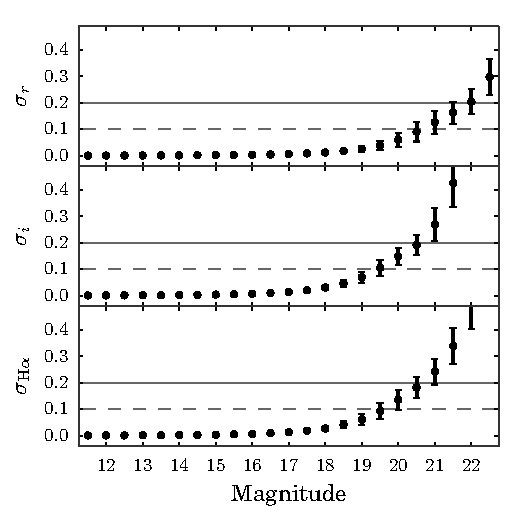
\includegraphics[width=0.5\textwidth]{figures/uncertainties/uncertainties.pdf} 
    \caption{Mean photometric uncertainties
             for $r$ (top), $i$ (middle) and \ha\ (bottom).
             Data points shown are the average values of
             columns \emph{rErr}, \emph{iErr} and \emph{haErr}
             in the catalogue 
             and the error-bars show the standard deviations.
             The dashed and solid lines indicate 
             the 10$\sigma$ and 5$\sigma$ limits, respectively.
             These statistics show the average level of the Poissonian
             photon noise and do not include systematic uncertainties.}
    \label{fig:uncertainties}
\end{figure}


Fig.~\ref{fig:uncertainties} shows the mean photometric
uncertainties (\emph{rErr}, \emph{iErr}, \emph{haErr})
as a function of magnitude.
We find the typical uncertainty to reach 0.1~mag near $r=$20.5 
and $i$/\ha$=19.5$.
We note that the fainter depth in $r$ is compensated
by the fact that most stars have brighter magnitudes in $i$ and \ha;
the average colours in the catalogue are
$\overline{(r-i)}=1.06\pm0.12$ and $\overline{(r-\ha)}=0.44\pm0.03$.
We warn that the statistics shown in Fig.~\ref{fig:uncertainties}
are the random errors based on the expected Poissonian photon noise.
Systematics, such as calibration and deblending errors,
are not included.

To appraise the level at which our photometry is affected by such systematics,
we can exploit the secondary measurements which are present in the catalogue
(i.e. \emph{r} vs \emph{r2}, \emph{i} vs \emph{i2}, \emph{ha} vs \emph{ha2}).
In Fig.~\ref{fig:pairmag} we show the mean absolute residuals between
these primary and secondary magnitudes as a function of magnitude (black dots).
We also plot the Poissonian uncertainties for comparison (solid red line).
We find the mean residual to equal $0.03\pm0.04$~mag
across the magnitude ranges 13 to 18 ($r$)
and 12 to 17 ($i$, \ha),
consistent with the accuracy of our calibration estimated above.
Stars fainter than this range appear to be dominated by photon noise (red line),
while stars at the bright end appear to suffer from large systematic
errors due to saturation effects.

\begin{figure*}
\captionsetup[subfigure]{labelformat=empty}
\begin{subfigure}[b]{0.45\linewidth}
\centering
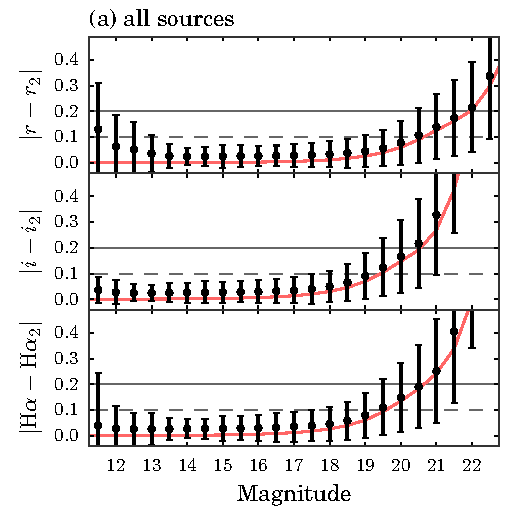
\includegraphics[width=\textwidth]{figures/repeatability/repeatability.pdf}
\caption{}
\label{fig:pairmag}
\end{subfigure}
\hspace{0.5cm}
\begin{subfigure}[b]{0.45\linewidth}
\centering
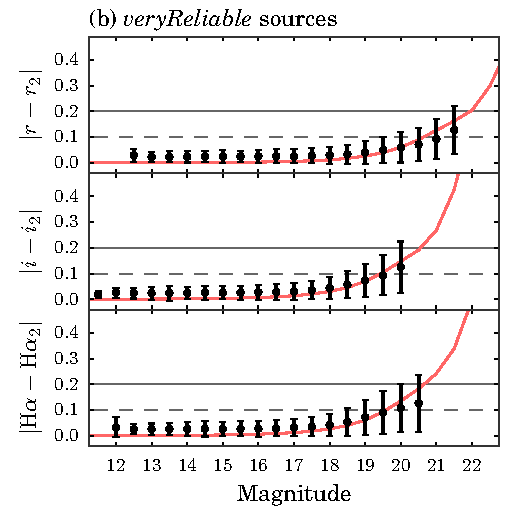
\includegraphics[width=\textwidth]{figures/repeatability/repeatability-reliable.pdf}
\caption{}
\label{fig:pairmag_reliable}
\end{subfigure}
\caption{Photometric repeatability as a function of magnitude
         for all sources in the catalogue (left panel)
         and for the \emph{veryReliable} sources alone (right panel).
         Black dots show the mean absolute residuals
         between the primary and the secondary detections.
         The error-bars show the standard deviations.
         The red trend line shows the average Poissonian uncertainties
         we derived in Fig.~\ref{fig:uncertainties}.
         We find that the \emph{veryReliable} quality criteria are successful
         at removing objects with large uncertainties.
    }
\end{figure*}

In Fig.~\ref{fig:pairmag_reliable} we show 
a similar comparison between the primary and secondary detections,
but this time we have only included sources which are flagged
as \emph{veryReliable} in the catalogue.
We do not observe an improvement in the average residuals as a function of magnitude,
but the number of outliers has decreased markedly
(evidenced by the shorter error bars which denote the standard deviation of the absolute residuals).
We conclude that the \emph{veryReliable} quality criteria are effective
at reducing the level of the systematic errors,
while also removing the unreliable data at the bright and faint end.

\subsection{Source counts and blending}
\label{sec:densities}

Fig.~\ref{fig:sourcecount} shows the number of sources
in the catalogue counted in $1^\circ$-wide strips
as a function of Galactic longitude (thick blue line).	
Unsurprisingly, we find the number of sources
to increase towards the Galactic centre.
For example, the average source density near $l\simeq 30^\circ$
is roughly 300\,000 objects per square degree,
which is six times more than the density
found near $l\simeq 180^\circ$.
In addition to the global trend,
variations are also apparent on smaller scales.
For example, we find a significant drop near the constellations 
of Aquila ($l\simeq40$) and Cygnus ($l\simeq80$ and $l\simeq90$),
which are regions known to be affected
by high levels of foreground extinction
\citep[the extremities of `the Great Rift', e.g.][]{BokBok}.
However, we warn that the source counts shown 
have not been corrected for field pairs that have yet
to be released or for variations in the depth across the included fields.
For example, the dip in the density near $l\simeq140^\circ$
is an artificial feature caused by gaps
in the footprint coverage (seen in Fig.~\ref{fig:footprint}).

In a forthcoming paper, properly calibrated maps of stellar density
of the northern Galactic Plane will be presented (Farnhill
et al., in preparation).  This will incorporate completeness
corrections based on the statistics of artificial source
recovery.  Such maps are of interest as tests of detailed models of 
our Galaxy.

\begin{figure*}
    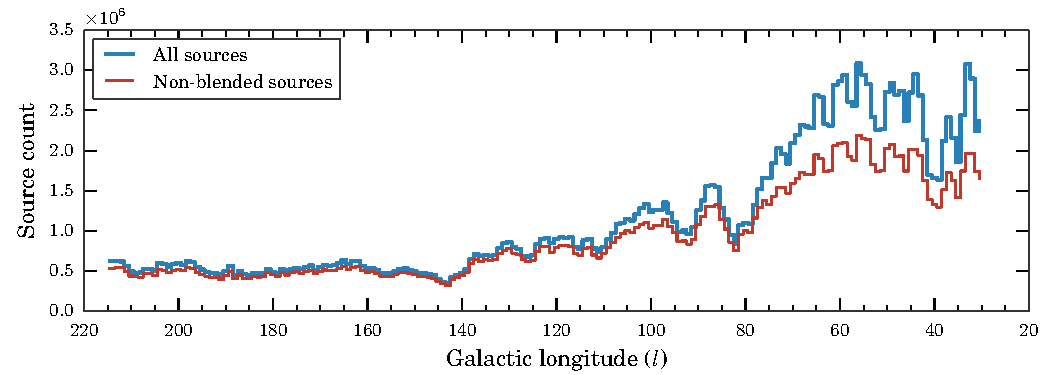
\includegraphics[width=\textwidth]{figures/sourcecount/sourcecount.pdf} 
    \caption{Number of entries in the IPHAS DR2 source catalogue
    as a function of Galactic longitude.
    The upper blue line shows the number of sources
    counted in 1\deg-wide longitude bins.
    The lower red line uses the same binning
    but includes only those sources 
    for which the \emph{deblend} flag is {\sc false}, 
    i.e. unconfused sources for which the CASU pipeline
    did not have to apply a deblending procedure.
    In both cases only counted sources
    in the latitude range $-5^\circ<b<+5^\circ$,
    such that one may obtain approximate source densities
    by dividing the counts by 10~deg$^2$.
    The apparent variations in the source counts
    traces the structure of the Galaxy
    and the distribution of foreground extinction,
    but also includes instrumental effects
	such as variations in the survey depth
	and completeness (see text).
   }
    \label{fig:sourcecount}
\end{figure*}

Fig.~\ref{fig:sourcecount} also shows the number counts
for non-blended sources (thin red line).
These are sources for which the \emph{deblend} flag is {\sc false},
i.e. sources for which the CASU pipeline did not have to apply 
a deblending procedure to separate the flux
originating from two or more overlapping objects.
This provides some insight into how the fraction of 
blend-affected sources correlates with the local source 
density.  In hard numbers, only 11\% of the sources are blended
at $l>90^\circ$, whereas 24\% are blended at $l<90^\circ$.

Finally, we warn that blended objects
are more likely than unblended objects to have fallen victim
to source confusion during the band-merging procedure.  It is
important to bear this in mind when appraising stars of seemingly
unusual colours (such as candidate emission line stars) -- if 
blending is flagged, the probability that the unusual colour is 
spurious is greatly increased.
%We have started investigating the use of
%more advanced PSF-fitting routines
%in which sources are measured simultaneously across all bands,
%which may be guided by an external astrometric catalogue
%such as the one that is to be provided by Gaia.

\section{Demonstration}
\label{sec:demonstration}

We conclude this paper by demonstrating how the unique
$(r-\ha,\ r-i)$ colour-colour diagram offered by this catalogue
can readily be used to
(i) characterise the extinction regime along different sight-lines, and
(ii) identify \ha\ emission-line objects.

\subsection{Colour-colour and colour-magnitude diagrams}

The survey's unique $(r-\ha)$ colour,
when combined with $(r-i)$,
has been shown to provide simultaneous constraints 
on intrinsic stellar colour and interstellar extinction \citep{Drew2008}. 
Put differently, the main sequence in the $(r-\ha,\ r-i)$ diagram
runs in a direction that is at a large angle relative to the reddening vector,
because the ($r-\ha$) colour tends to act
as a coarse proxy for spectral type
and is less sensitive to reddening than $(r-i)$.
As a result, the distribution of a stellar population
in the IPHAS colour-colour diagram
can offer a handle on the properties of the population
and the extinction along a line of sight.

This is demonstrated 
in Fig.~\ref{fig:l180}, \ref{fig:l45} \& \ref{fig:l30},
where we present three sets of IPHAS colour/magnitude diagrams
towards three distinct sight-lines
located at Galactic longitudes 
$180^\circ$, $45^\circ$ and $30^\circ$, respectively.
Each figure contains all the sources
flagged as \emph{veryReliable} within a region of one square degree 
centred on the coordinates indicated in the diagram
(i.e. within a radius of $0.564^\circ$ from the indicated sight-line).
For clarity, we have imposed the additional criterion
that the photometric uncertainties
must be smaller than 0.05 mag in each band,
corresponding to a magnitude limit near $\sim$19th magnitude.

Each of the diagrams reveal a well-defined locus,
which helps to demonstrate the health of the catalogue and the 
global calibration
for investigating stellar populations across wide areas.
We have annotated the colour-colour diagrams
by showing the position 
of the unreddened main sequence (thin solid line),
the unreddened giant branch (thick solid line),
and the reddening track for an A0V-type star (dashed line)
-- all three are based on the \cite{Pickles1998} library 
of empirical spectra
transformed into the Vega-based IPHAS system by \cite{Drew2005}.
In the colour-magnitude diagrams we only show the reddening vector
together with the unreddened 1~Gyr isochrone due to \cite{Bressan2012},
which is made available for the IPHAS system through the
on line tool hosted at the Observatory of Padova
(http://stev.oapd.inaf.it/cmd).
The isochrone and reddening vector have been placed
at an arbitrary distance of 2~kpc.

Each of the sightlines reveal a stellar population
with distinct characteristics.
Towards the Galactic anti-centre 
at $l=180^\circ$ (Fig.~\ref{fig:l180})
we find a population dominated by lowly-reddened main sequence stars.
This is consistent with the estimated total sight-line extinction 
of $E(B-V)=0.49$ given by \cite{Schlegel1998},
following the correction of \cite{Schlafly2011}.
Looking in more detail we can see
that the stellar locus is narrower for M-type dwarfs
than for earlier types;
we do not observe M dwarfs experiencing 
the strongest reddening possible for this sight-line.
This implies that extinction is still increasing 
at distances of $\sim$1-2~kpc,
where M dwarfs become too faint to be contained in the IPHAS catalogue.
It is also clear that there are no unreddened stars
earlier than $\sim$K0 visible;
such stars would be saturated if within a few hundred parsecs.
This therefore suggests 
that there is a measurable increase in extinction locally.
We also note a relative absence of late type giants which,
due to the relative brevity 
of the corresponding phase of stellar evolution,
would only account for a small proportion of the more nearly volume 
limited sample seen in the Anticentre direction.
 
In contrast, 
closer towards the galactic centre
at $l=45^{\circ}$ (Fig.~\ref{fig:l45}),
there is  a wealth of reddened objects.
In the colour-magnitude diagram, it is clear
that the stars are split into two distinct groups,
with one significantly redder than the other.
The bluer group is composed of main sequence stars,
with the slope of this group in the colour-magnitude diagram
attributable to the significantly increasing extinction.
Meanwhile the redder group is principally composed of red giant stars \citep[see][]{Wright2008}.
As these stars are intrinsically brighter, they will be substantially 
further away than their main sequence counterparts at the same 
apparent magnitude.  Given that extinction continues to increase 
with distance, along this sightline, 
the red giants we observe will be subject to appreciably more reddening
than the main sequence stars, pushing them to $r - i \sim 1.5$.


Finally, in one of our earliest sight-lines at $l=30^{\circ}$,
we find a very high number of extremely reddened giants
in addition to an unreddened population
of foreground dwarfs.
In contrast to the sight-line at $l=45^{\circ}$,
there is no clear group of giant stars visible
in the colour-magnitude diagram of Fig.~\ref{fig:l30},
although the red clump stars are manifest as a track of slight 
over density sitting roughly 0.4~mags redder than the A0V reddening track.
At $(l,b)=(45^{\circ}, +2^{\circ})$ the giant stars observed
exhibit a relatively narrow range of reddenings
as they lie beyond most or essentially all of the Galactic dust.
At $(l,b)=(30^{\circ}, 0^{\circ})$ this is not the case:
even at the substantial distances
at which we can observe reddened giant stars,
extinction is continuing to rise within the Galactic mid-plane.
It is also apparent that the $(r-i)$ width of both the M dwarfs
and early A dwarfs is greater than that in Fig.~\ref{fig:l45}.
This is indicative of a steeper rise in reddening,
both within several hundred parsecs (M dwarfs)
and within a few kpc (early A dwarfs).

These are just qualitative vignettes of the information obtainable
from IPHAS colour-colour and colour-magnitude plots.
A more rigorous quantitative analysis of the IPHAS catalogue
can be undertaken to estimate both the stellar density distribution 
in the Milky Way \citep{Sale2010} and to create detailed three-dimensional 
maps of the extinction across several kpc \citep{Sale2009,Sale2012}.
A 3-D extinction map based on the DR2 catalogue
is being released in a separate paper (Sale et al., in preparation).

\begin{figure*}
    \begin{minipage}[b]{\linewidth}
        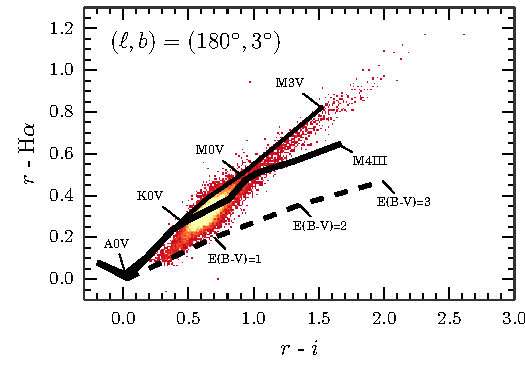
\includegraphics[width=0.5\textwidth]{./plots/ccd-180-3.pdf} 
        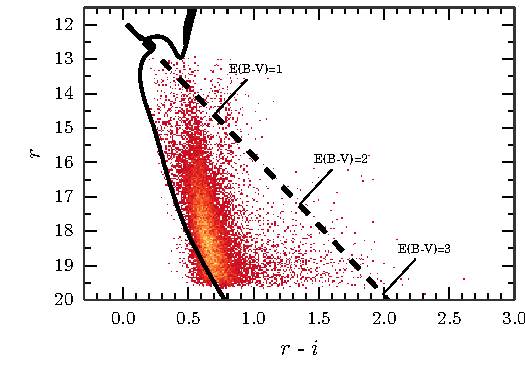
\includegraphics[width=0.5\textwidth]{./plots/cmd-180-3.pdf}
    \end{minipage}
    \caption{Colour-colour and colour-magnitude diagrams
    (left and right panel)
    showing sources flagged as \emph{veryReliable}
    located in an area of one square degree
    centred near the Galactic anti-centre 
    at $(l,b)=(180^\circ,+3^\circ)$.
    The diagrams are plotted as 2D-histograms
    which show the density of objects
    in bins of $\sim0.01\times0.01$~mag;
    bins containing 1-10 objects are coloured red,
    bins with 10-20 objects are orange,
    and bins with 20-25 objects are yellow.
    The left panel is annotated with
    the position of the main sequence (thin solid line),
    giant stars (thick solid line)
    and the reddening track for an A0V-type star (dashed line),
    which are based on the \citet{Pickles1998} library
    of observed spectra.
    The right panel only shows the reddening vector
    along with the unreddened 1~Gyr isochrone due to \citet{Bressan2012},
    which has been placed at an arbitrary distance of 2~kpc.
    This is one of the least reddened sight-lines
    in the survey
    and hence the observed stellar population appears to be dominated 
    by lowly reddened main sequence stars (see text).}
    \label{fig:l180}
    \begin{minipage}[b]{\linewidth}
        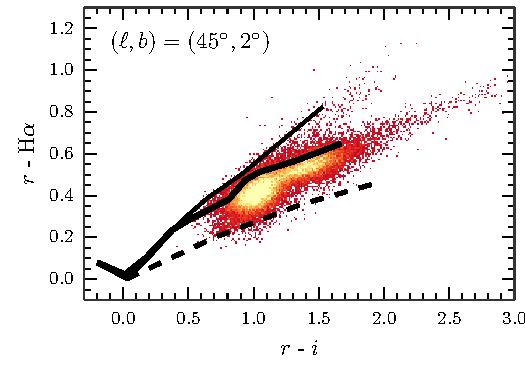
\includegraphics[width=0.5\textwidth]{./plots/ccd-45-2.pdf}
        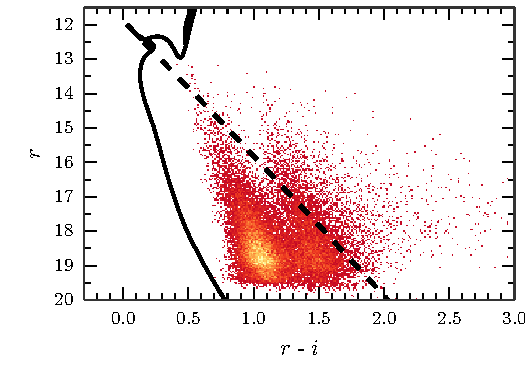
\includegraphics[width=0.5\textwidth]{./plots/cmd-45-2.pdf}
    \end{minipage}
    \caption{Same as above for $(l,b)=(45^\circ,+2^\circ)$,
    which is one of the highest-density sight-lines in the survey,
    revealing two groups of stars in colour-magnitude space.}
    \label{fig:l45}
    \begin{minipage}[b]{\linewidth}
        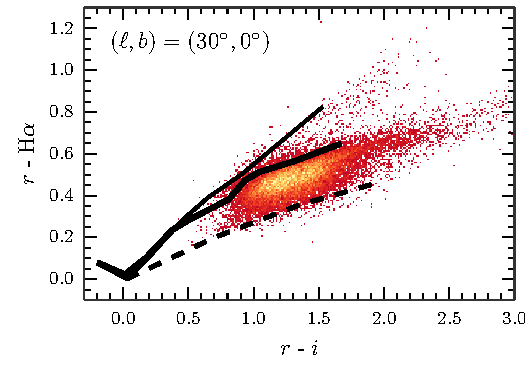
\includegraphics[width=0.5\textwidth]{./plots/ccd-30-0.pdf}
        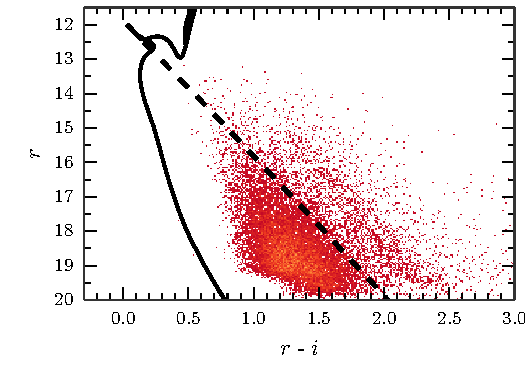
\includegraphics[width=0.5\textwidth]{./plots/cmd-30-0.pdf} 
    \end{minipage}
    \caption{Same as above for $(l,b)=(30^\circ,0^\circ)$,
    showing one of the most reddened sight-lines in the survey.
    }
    \label{fig:l30}
\end{figure*}

\subsection{Identifying \ha\ emission-line objects}

An aim of IPHAS is to enable the discovery 
of new fainter emission-line objects
across the Galactic Plane.
\ha\ in emission is a well-known tracer
for stars in the short-lived pre- or
post-main sequence stages of their evolution,
and hence IPHAS allows larger, deeper
and more statistically robust samples
of such rare objects to be established.
The survey-wide identification and analysis 
of emission-line objects is beyond the scope
of the present work and will be the focus
of a forthcoming paper (Barentsen et al, in preparation).
In this section we merely aim to demonstrate
a use of the catalogue for this purpose.

An initial list of candidate \ha-emitters
based on the first IPHAS data release was previously
presented by \cite{Witham2008}. 
Because no uniform calibration was available
at the time, \citeauthor{Witham2008} employed 
a sigma-clipping technique to select objects with
large, outlying $(r-\ha)$ colours.
In contrast, the new catalogue
allows objects to be picked out
from the $(r-\ha,\ r-i)$ colour-colour diagram
using model-based colour criteria
rather than a statistical procedure.
In what follows we demonstrate this ability 
by selecting candidate emission-line objects
towards a small region in the sky.

The target of our demonstration is Sh 2-82:
a 5~arcmin-wide H{\sc ii} region located near $(l,b)=(53.55^\circ, 0.00^\circ)$
in the constellation of Sagitta.
Nicknamed by amateur astronomers as the `Little Cocoon Nebula',
Sh 2-82 is ionised by 
the $\sim$10th magnitude star HD\,231616
with spectral type B0V/III
\citep{Georgelin1973,Mayer1973,Hunter1990}.
This ionising star has been placed 
at a likely distance of 1.5-1.7 kpc
based on its photometric parallax
\citep{Mayer1973,Lahulla1985,Hunter1990}.

Fig.~\ref{fig:mosaic_iphas} shows a 20-by-15 arcmin
colour mosaic centred on Sh 2-82,
composed of our \ha\ (red channel),
$r$ (green channel),
and $i$ (blue channel) images.
The ionising star can be seen as the bright object
in the centre of the H{\sc ii} region,
which is surrounded by a faint reflection nebula
and several dark cloud filaments.
For comparison, Fig.~\ref{fig:mosaic_spitzer} shows
a mosaic of the same region 
as seen in the mid-infrared by the Spitzer Space Telescope \citep[GLIMPSE survey;][]{Benjamin2003,Churchwell2009}.
The infrared image reveals an enclosing fuzzy bubble (appearing
green in Fig.~\ref{fig:mosaic_spitzer})
which is thought to originate from the
mid-infrared emission of Polycyclic Aromatic Hydrocarbons (PAHs)
-- i.e. warm dust --
which is frequently observed
at the interface between neutral regions of interstellar material
and the ionising radiation from early-type stars \citep{Churchwell2006}.
\cite{Yu2012}
recently noted that the warm dust
that surrounds Sh~2-82 
appears to contain infrared-bright
Young Stellar Objects (YSOs).
Many of these young objects 
appear as red- and pink-coloured stars
in Fig.~\ref{fig:mosaic_spitzer},
located predominantly in the top-left part
of the bubble.

\begin{figure*}
    \begin{minipage}[b]{0.78\linewidth}
        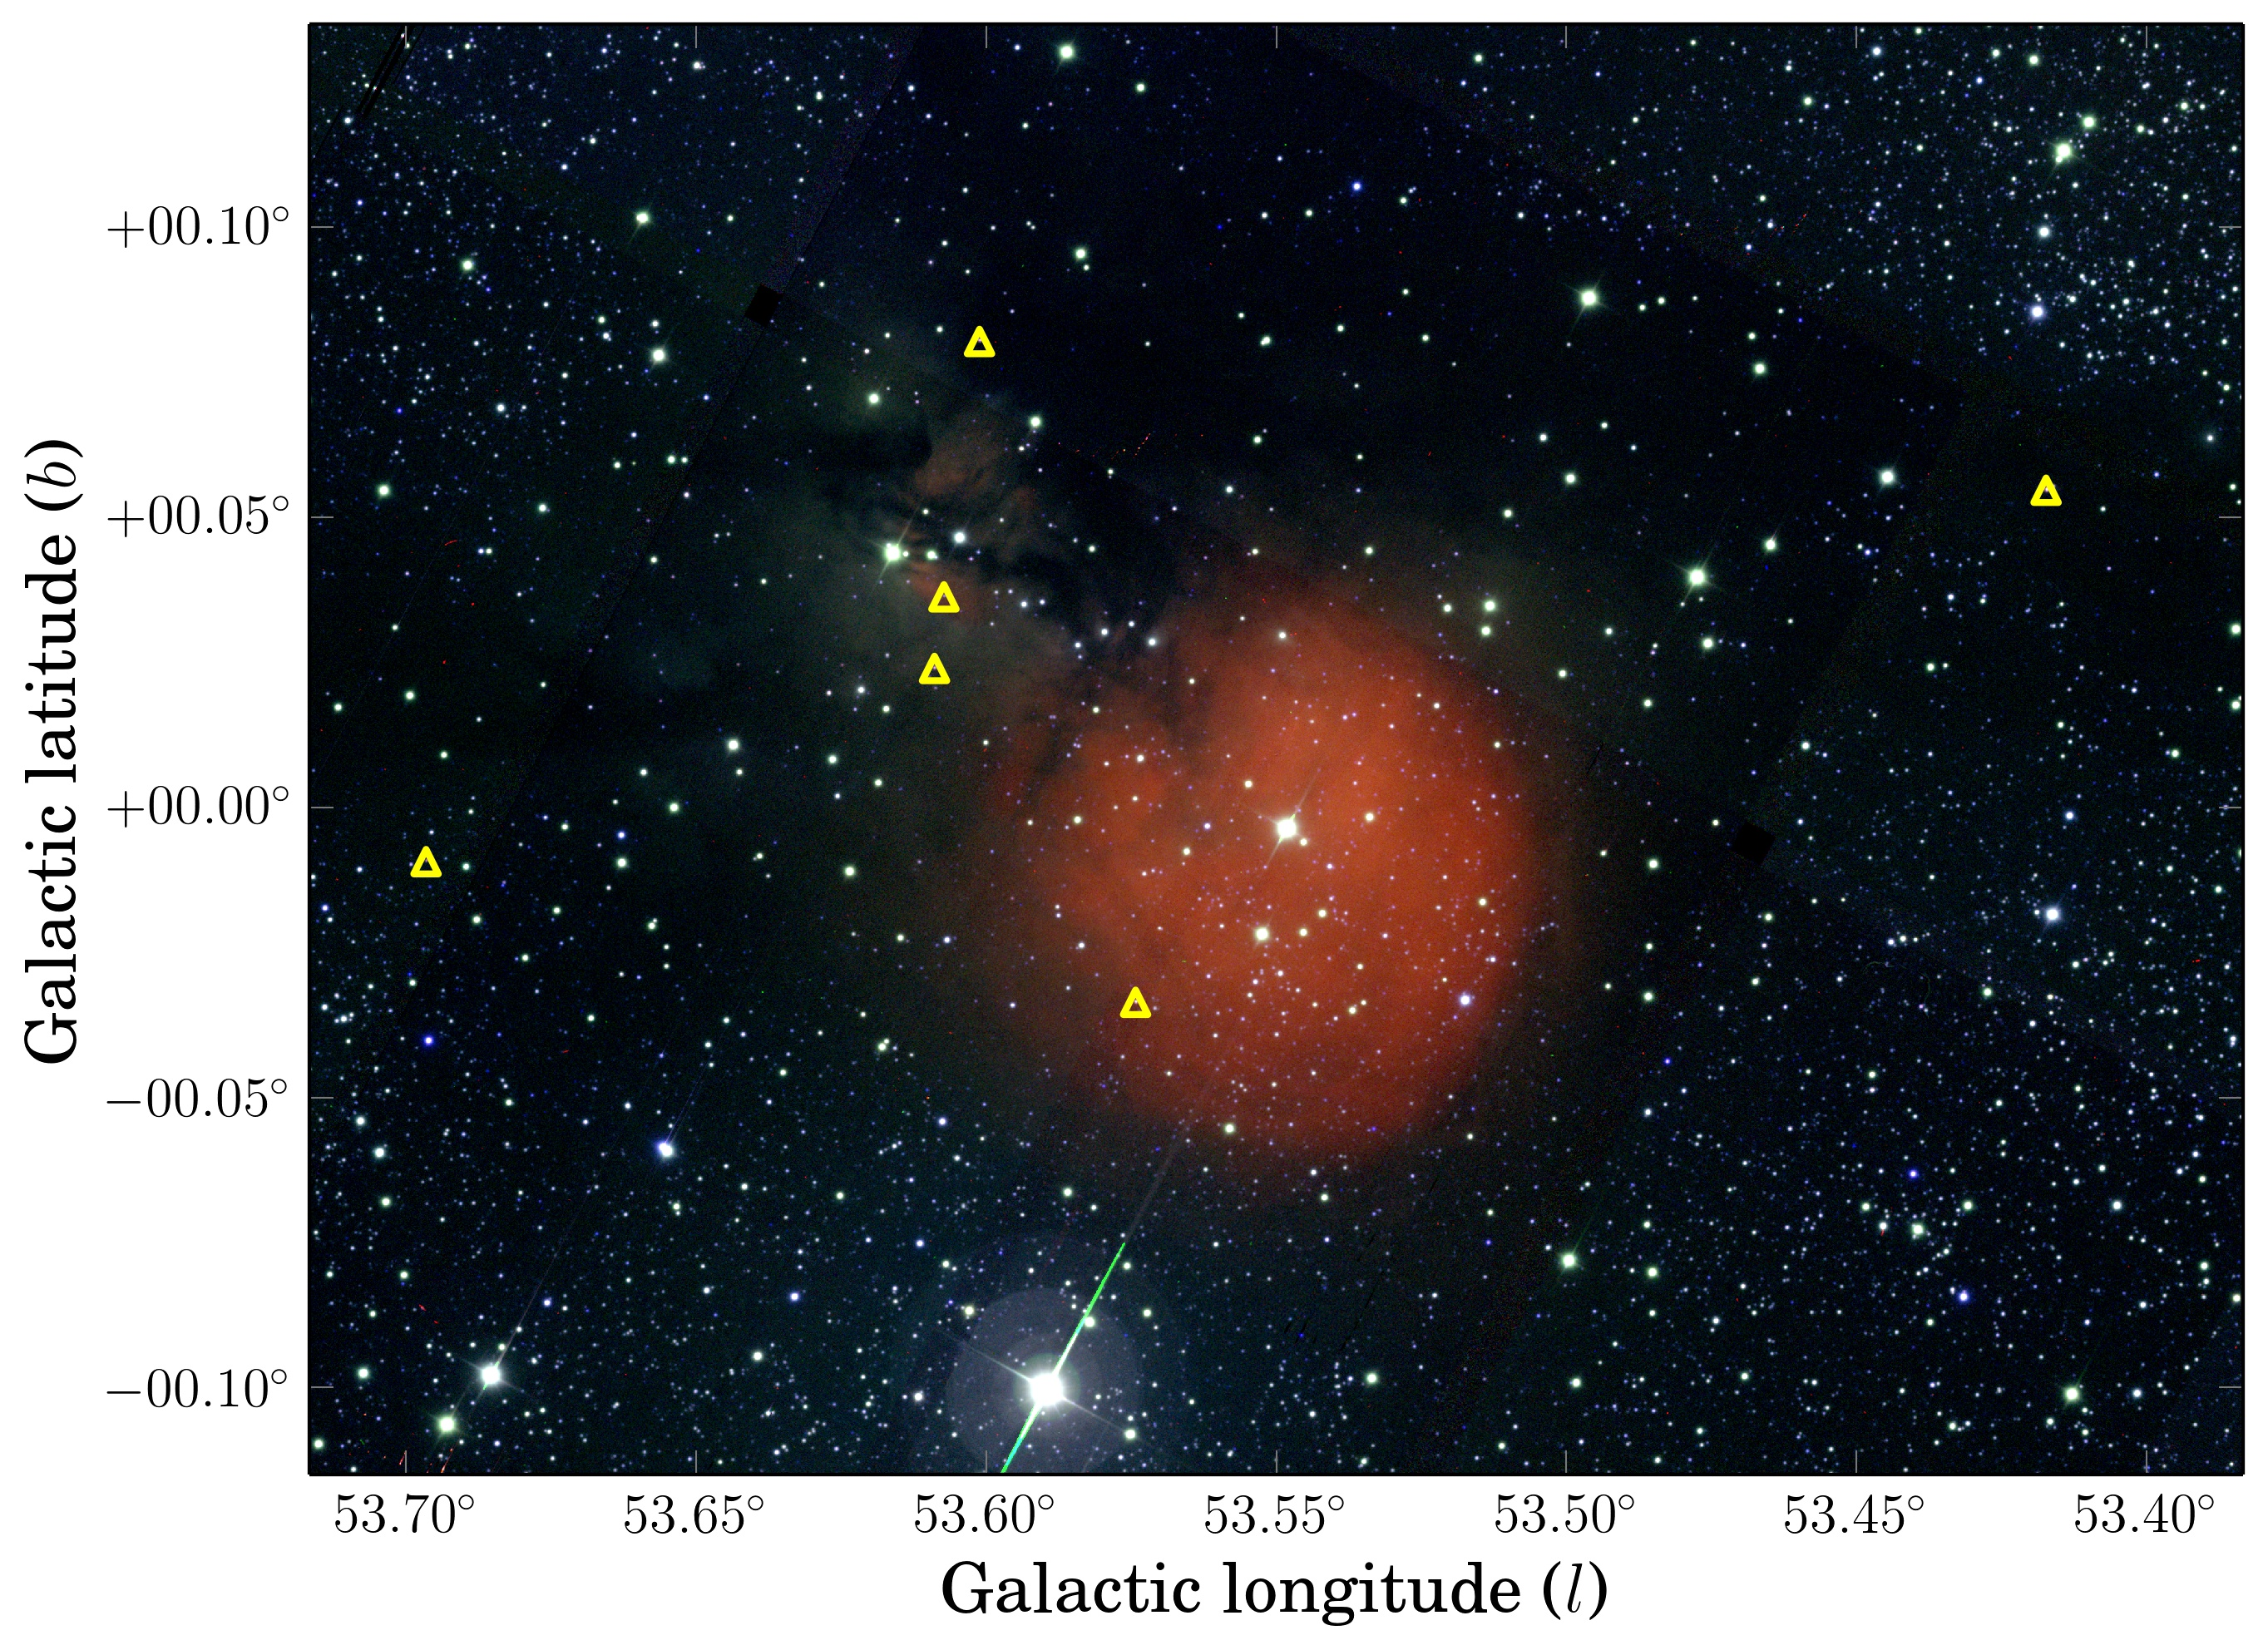
\includegraphics[width=\textwidth]{./plots/mosaic/sh2-82-iphas.pdf} 
    \end{minipage}
\caption{IPHAS-based mosaic of H{\sc ii} region Sh 2-82,
composed of \ha\ (red channel), $r$ (green channel) and $i$ (blue channel). Yellow triangles show the position of candidate \ha-emitters
which have been selected from the colour-colour diagram
in Fig.~\ref{fig:emitters}. Note that the H{\sc ii} region is surrounded by a faint blue/green reflection nebula
and dark cloud filaments.}
\label{fig:mosaic_iphas}
    \begin{minipage}[b]{0.78\linewidth}
        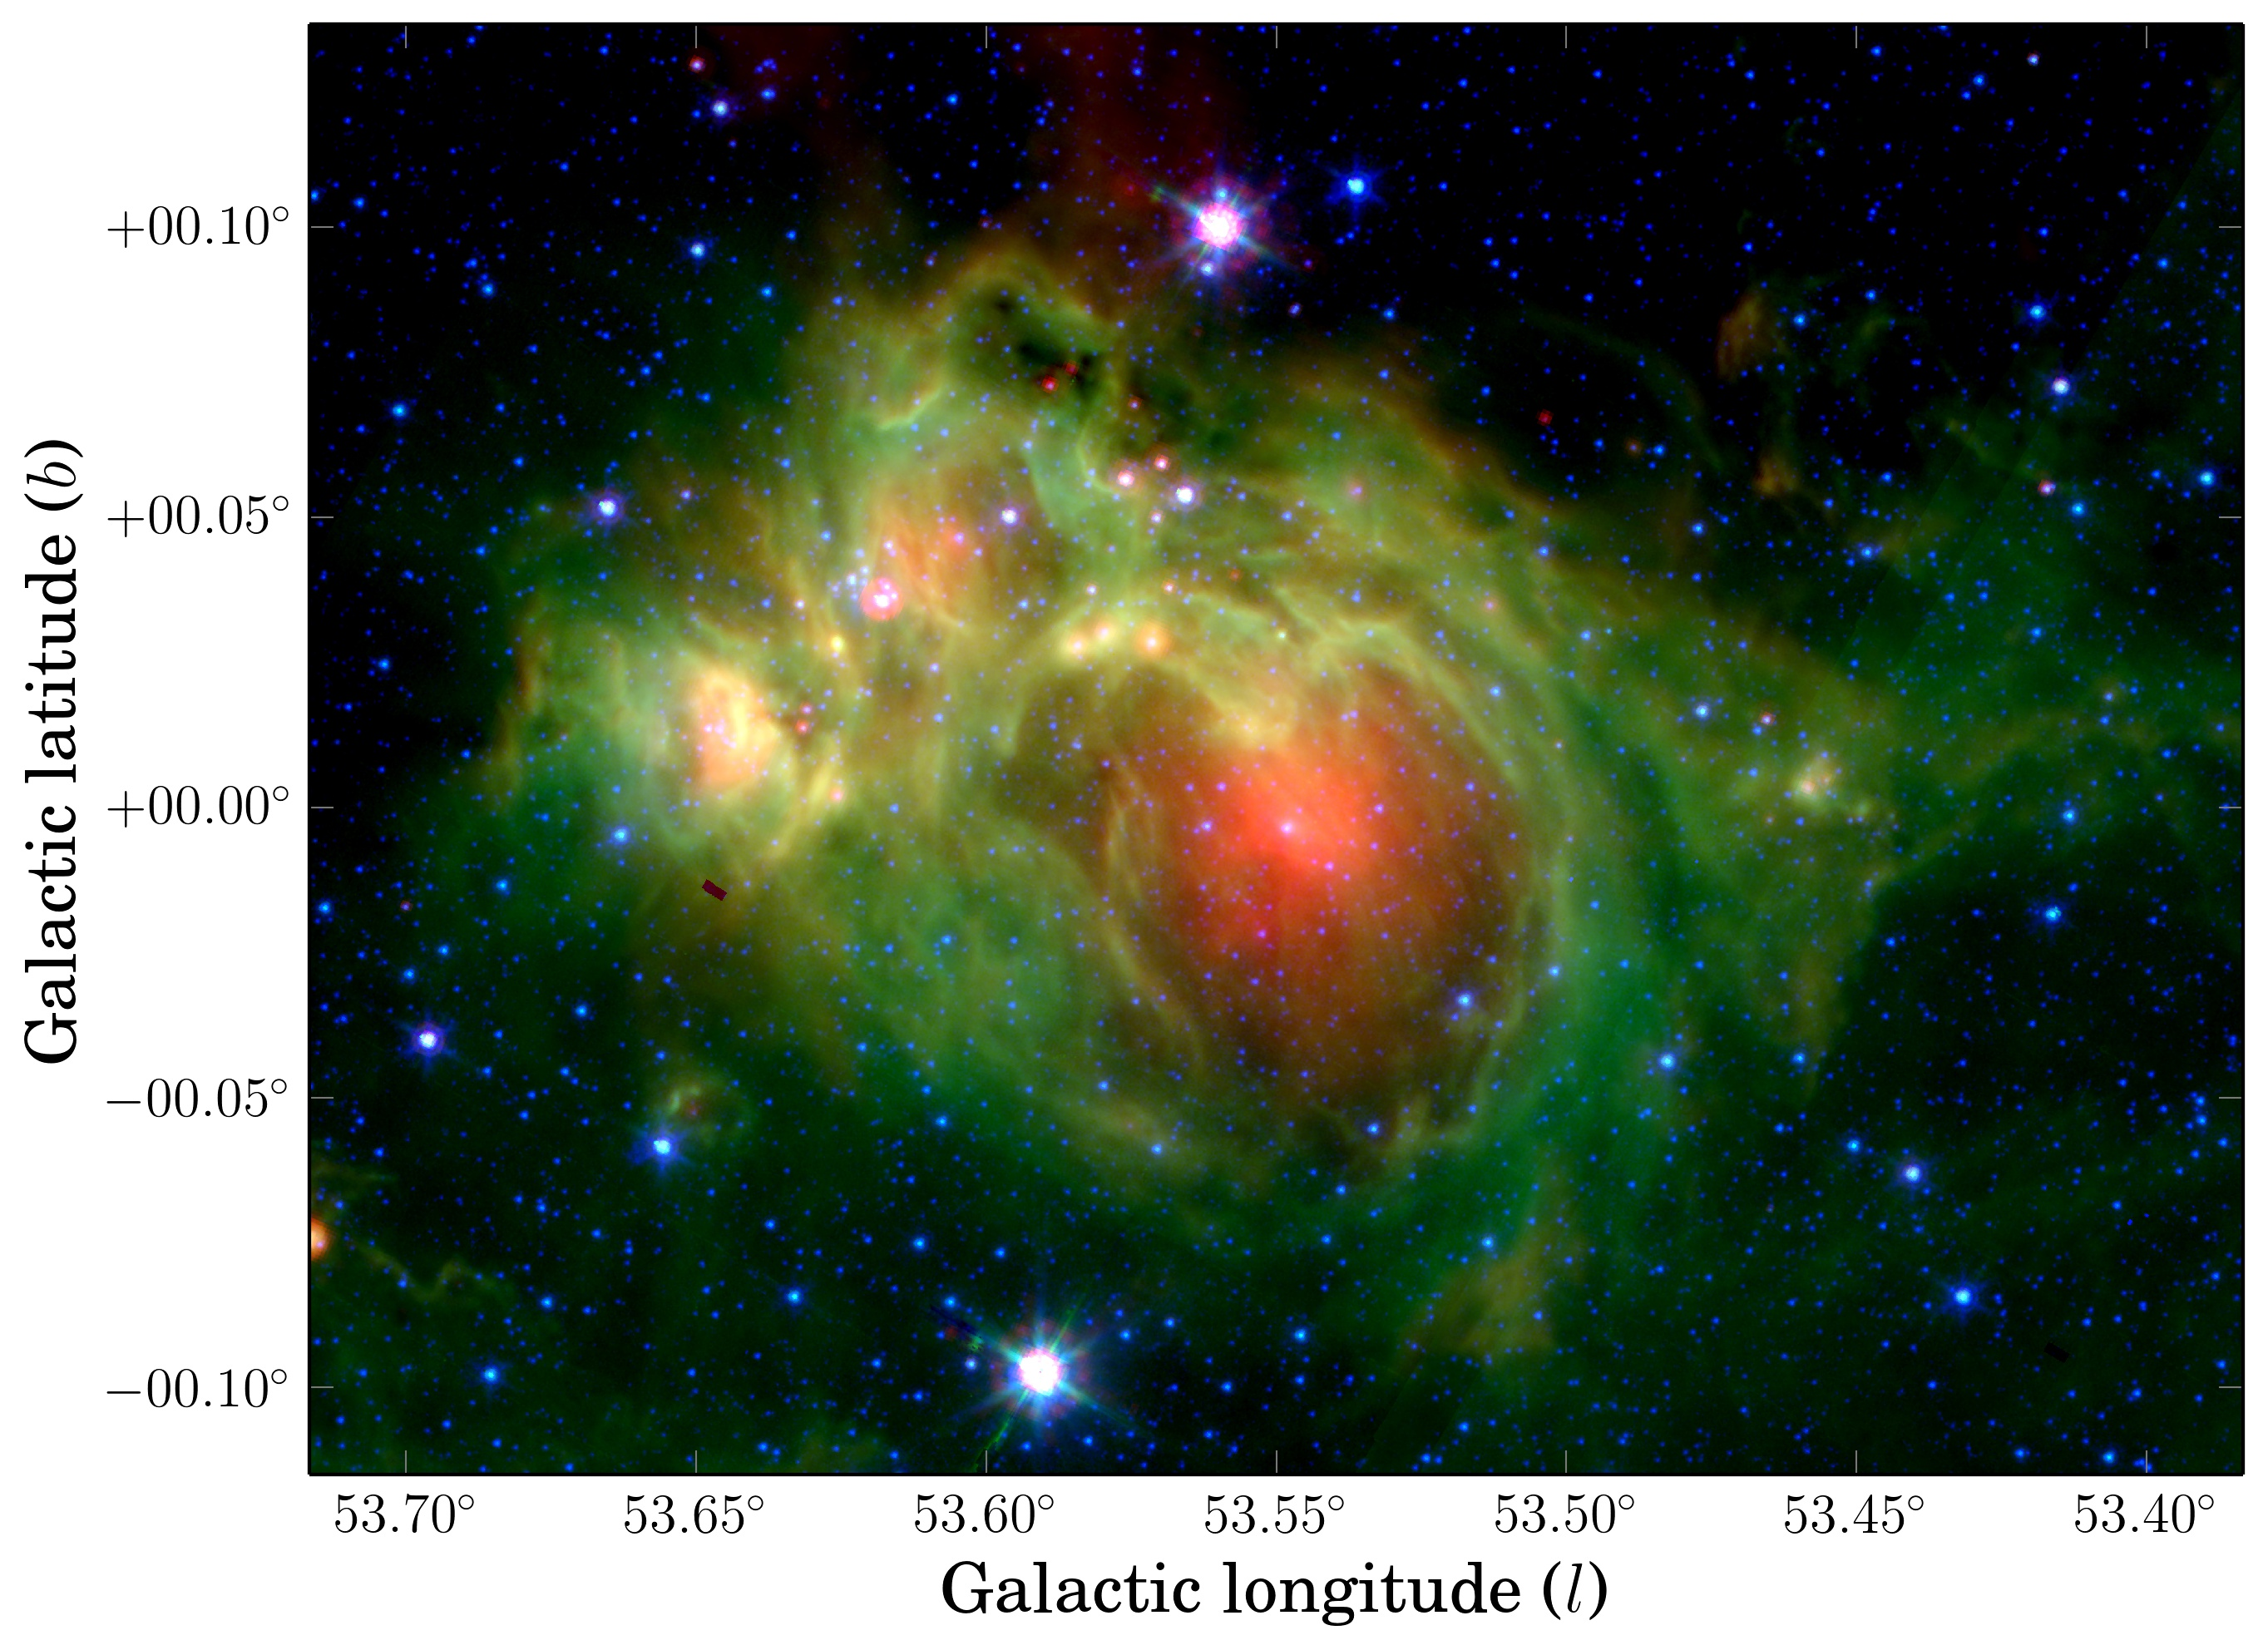
\includegraphics[width=\textwidth]{./plots/mosaic/sh2-82-spitzer.pdf} 
    \end{minipage}
    \caption{Star-forming region Sh 2-82 as seen in the mid-infrared
    by the Spitzer Space Telescope. The mosaic is composed of the 24~\micron\ (red), 8.0~\micron\ (green) and 4.5~\micron\ (blue) bands.
    The image reveals a bubble-shaped structure which surrounds the {\sc Hii} region that is seen in the IPHAS mosaic which spans the same region (Fig.~\ref{fig:mosaic_iphas}). 
    This structure has previously been labelled as N115 in the 
catalogue due to \citet{Churchwell2006}, and could be a possible site of triggered star formation \citep{Thompson2012,Kendrew2012}.}
    \label{fig:mosaic_spitzer}
\end{figure*}

Fig.~\ref{fig:emitters} presents
the IPHAS colour-colour diagram for 
the 20-by-15 arcmin region shown in the mosaics.
Gray circles show all objects
which are brighter than $r<20$
and have been flagged as \emph{reliable}
in our catalogue.
The diagram also shows the unreddened main sequence (solid line)
and the expected position of unreddened main-sequence stars
with \ha\ in emission
at a strength of EW$=-10$~\AA\ (dashed line).
Six stars are found to lie above the 
dashed line at the level of $3\sigma$,
i.e. the distance between the objects and the dashed line
is larger than three times the uncertainty
in their $(r-\ha)$ colour.
These candidate \ha-emitters
are marked by red triangles in the colour-colour diagram,
and yellow triangles in the image mosaic (Fig.~\ref{fig:mosaic_iphas}).
Their details are listed in Table~\ref{tbl:emitters}.

\begin{figure}
  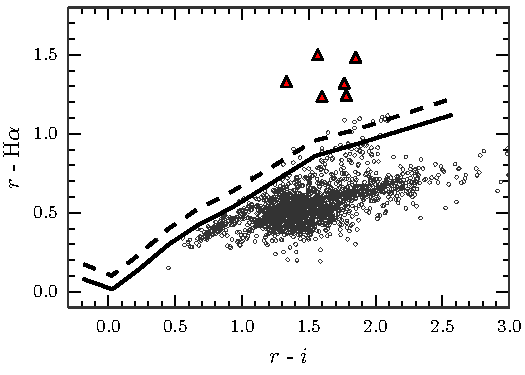
\includegraphics[width=0.45\textwidth]{./plots/sh2-82-ccd.pdf}
    \caption{$(r-\ha,\ r-i)$ diagram for the rectangular region of 
    20-by-15 arcmin centred on the H{\sc ii} region Sh 2-82,
    which is the area shown in Fig.~\ref{fig:mosaic_iphas}.    
    The diagram shows all objects in the catalogue
    which have been flagged as \emph{reliable} and are brighter
    than $r<20$ (grey circles).
    The unreddened main sequence is indicated by a solid line,
    while the main sequence for stars with an \ha\ emission line
    strength of $-10~\rm{\AA}$~EW is indicated by a dashed line
    \citep[both based on the colour simulations by][]{Barentsen2011a}.
    Red triangles indicate objects which have been identified as
    as likely \ha-emitters.}
    \label{fig:emitters}
\end{figure}

\begin{table}
    \caption{Candidate \ha-emitters towards Sh 2-82.}
    \label{tbl:emitters}
    \footnotesize
    \resizebox{0.45\textwidth}{!}{
        \begin{tabular}{clccc}
        \toprule
        \# & Name [IPHAS2 ...] & $r$ & $i$ & \ha  \\
        \midrule
        1 & J192954.40+181026.1& $17.69\pm0.01$ & $16.12\pm0.01$ & $16.19\pm0.01$ \\
        2 & J193011.01+182051.2& $18.55\pm0.02$ & $16.95\pm0.02$ & $17.31\pm0.02$ \\
        3 & J193021.52+181954.5& $19.72\pm0.05$ & $17.94\pm0.03$ & $18.47\pm0.04$ \\
        4 & J193024.45+181938.3& $19.31\pm0.04$ & $17.55\pm0.02$ & $17.99\pm0.03$ \\
        5 & J193033.00+181609.3& $18.25\pm0.01$ & $16.91\pm0.01$ & $16.92\pm0.01$ \\
        6 & J193042.48+182317.4& $19.96\pm0.03$ & $18.11\pm0.03$ & $18.48\pm0.03$ \\
        \bottomrule
        \end{tabular}
    }
\end{table}

In previous work, we have shown that the majority of
\ha-emitters seen by IPHAS towards an H{\sc ii} region
are likely to be Classical T Tauri Stars \citep{Barentsen2011a}.
These are young objects
which are thought to show \ha\ in emission
due to the presence of hot, infalling gas
which is accreting onto the star
from a circumstellar disk.
This is likely to be the case for the candidate \ha-emitters
we discovered towards Sh 2-82 as well.
Two of our candidates, \#1 and \#4 in Tab.~\ref{tbl:emitters},
have previously been identified
as candidate YSOs by \cite{Robitaille2008}
and \cite{Yu2012}, respectively.
In these studies, the authors used Spitzer data
to select intrinsically red objects,
which is consistent with the presence of a circumstellar disk.
Although the other four candidate emitters in our sample
have not previously appeared in the literature,
we note that all four are detected
in the Spitzer 8.0~\micron\ image at S/N$>$5.
They are likely to be Class II YSOs exhibiting a mild infrared excess.

Sh 2-82 is one of a large population of poorly-studied star-forming regions
located at low Galactic latitudes,
which have only recently started to become revealed
by efforts to catalogue the wealth of `bubbles' detected
at mid-infrared wavelengths \citep{Churchwell2006,Simpson2012},
and by efforts to catalogue previously unknown clusters seen 
in the near-infrared \cite[e.g.][]{Bica2003}.
IPHAS data can offer a handle
on the extinction, distance
and stellar contents of these unexplored regions.

\section{Data access and source code}
\label{sec:dataaccess}

The catalogue is made available through the Vizier
catalogue tool (http://vizier.u-strasbg.fr)
where it can be queried
(Conesearch/TAP URL TBD).
The catalogue can also be downloaded in its entirety
from the IPHAS website (www.iphas.org) as a collection 
of binary FITS tables occupying 50~GB,
together with a script
to ingest these tables into a PostgreSQL database.

The website also provides access to the pipeline-processed
imaging data, which we have updated to include
the re-calibrated zeropoints and the best-available
astrometric solution in the image headers.

In the spirit of reproducibility,
the source code that was used to generate
the catalogue is made available at
https://github.com/barentsen/iphas-dr2

Instructions for acknowledging IPHAS can be found on our website.


\section{Concluding remarks and future work}
\label{sec:conclusions}

A new catalogue of 219 million sources has been
derived from the INT/WFC Photometric \ha\ Survey
of the Northern Galactic Plane.
It is the first catalogue to offer comprehensive CCD photometry
of point sources across the Northern Galactic Plane at visible wavelengths,
taking in the latitude range $|b|<5^\circ$.
The new 98-column catalogue provides single-epoch photometry
across 92\% of the survey area,
and is the first quality-controlled and uniformly calibrated
catalogue to have been constructed from the imaging data.  This
now means that there is H$\alpha$ coverage, accessible online,
of the entire Galactic Plane -- given that the 
southern Plane is already available thanks to the UK
Schmidt H$\alpha$ Survey \citep[SHS,][]{Parker2005}, the last of the 
photographic surveys carried out by that telescope.

The observations included in this release
achieve a median seeing of 1.1 arcsec
and $5\sigma-$depths of $r=21.2\pm 0.5$, $i=20.0\pm 0.3$, and \ha$=20.3\pm 0.3$.
The global calibration and photometric repeatability
are found to be accurate at the level of $0.03$ mag (rms),
providing a significant improvement over the 
previous data release.
The source catalogue specifies the best-available
single-epoch astrometry and photometry
for 219~million unique sources.
To support its exploitation, we provide a list of recommended quality criteria
that will permit the selection of objects with reliable colours from 
the catalogue.  The closing demonstrations highlight the use of the 
survey's unique $(r-\ha,\ r-i)$ diagram for characterising stellar populations
and selecting emission-line objects.  More comprehensive applications of IPHAS
can be found in the works of Sale et al (2014), which applies DR2 to the problem
of 3D extinction mapping, and of Sabin et al (2014), where the results of a search
of the image database for new planetary nebulae is presented. 

The current plan is to work toward one further major IPHAS source catalogue, in which 
the remaining gaps in sky coverage will have been eliminated -- observations aimed at 
replacing data not meeting the IPHAS minimum quality requirements are continuing.  We will also 
examine options to further improve the global calibration, perhaps tightening the accuracy to
better than 2\%.  For example, we have in mind investigating the use of the PanSTARRS photometric 
ladder (Magnier et al 2013) as a reference set, when it becomes available and we will 
explore improving source recovery in 
the most dense fields via the implementation of PSF fitting in place of aperture photometry.  
Finally, the next catalogue will detail all the secondary detections to aid time-domain 
studies.

The data-taking strategy developed for IPHAS
has since been reapplied to carry out 
a companion INT/WFC Galactic Plane survey called UVEX
in U, $g$, $r$, He {\sc i} \citep{Groot2009},
a survey of the Kepler field 
in $U$, $g$, $r$, $i$, \ha\ 
\citep{Greiss2012},
and a survey of the Southern Galactic Plane and Bulge
in $u$, $g$, $r$, $i$, \ha\ 
called VPHAS+ \citep{Drew2014}.  The last of these incorporates the
digital update of the SHS, offering all the advantages of calibrated
photometry across a little over half the SHS footprint.  
The work presented here
stands as a potential template for the catalogues that
remain to be generated from these sibling surveys.  
In prospect from them, whether they are mined separately or together,
are the means to ask seamless questions on the contents and structure of 
the most highly-populated components of the Milky Way.  

\section*{Acknowledgments}

The INT is operated on the island of La Palma
by the Isaac Newton Group
in the Spanish Observatorio del Roque de los Muchachos
of the Instituto de Astrofisica de Canarias.
We are deeply indebted to the ING staff and students
for their ongoing support.
All data were processed 
by the Cambridge Astronomical Survey Unit
at the Institute of Astronomy in Cambridge.
The catalogue presented in this work was assembled
at the Centre for Astrophysics Research, University of Hertfordshire, supported by a grant from the Science \& Technology Facilities Council
of the UK (STFC, ref ST/J001335/1).

Preparation of the catalogue was eased greatly
by a number of software packages,
including the {\sc postgresql} database software,
the {\sc topcat} and {\sc stilts} packages \citep{Taylor2005,Taylor2006},
and the Python modules
{\sc astropy} \citep{Astropy},
{\sc numpy} and {\sc scipy} \citep{Numpy},
{\sc matplotlib} \citep{Matplotlib},
{\sc ipython} \citep{IPython},
and {\sc aplpy}.
We also made use of the {\sc montage} software maintained by NASA/IPAC,
and the {\sc simbad}, {\sc vizier} and {\sc aladin} services
operated at CDS, Strasbourg, France \citep{Aladin}.

Our work made extensive use of
several complementary photometric surveys.
Our global calibration was aided
by the AAVSO Photometric All-Sky Survey (APASS),
funded by the Robert Martin Ayers Sciences Fund.
The calibration was tested against the
Sloan Digitized Sky Survey (SDSS),
funded by the Alfred P. Sloan Foundation,
the Participating Institutions,
the National Science Foundation,
the U.S. Department of Energy,
the National Aeronautics and Space Administration,
the Japanese Monbukagakusho, the Max Planck Society,
and the Higher Education Funding Council for England.
The astrometric pipeline reduction made
significant use of the Two Micron All Sky Survey (2MASS),
which is a joint project 
of the University of Massachusetts
and the Infrared Processing and Analysis Center/
California Institute of Technology,
funded by NASA and the NSF.
This work includes observations made
with the Spitzer Space Telescope,
which is operated by the Jet Propulsion Laboratory,
California Institute of Technology under a contract with NASA. 

GB, JED, SES and BTG acknowledge support from the Science \& Technology
Facilities Council of the United Kingdom
(grants: GB and JED ST/J001333/1, SES ST/K00106X/1, BTG ST/I001719/1). 
HJF is in receipt of an STFC postgraduate studentship.  JED would also
like to convey her thanks to the Physics Department of Imperial College
London that hosted this project from its inception to 2007 and supported
her via a sabbatical year in 2003-4.  BTG acknowledges funding from the
European Research Council under the European Union's Seventh Framework
Programme (FP/2007-2013) / ERC Grant Agreement n. 320964 (WDTracer).
NJW is in receipt of a Fellowship funded by the Royal Astronomical Society
of the United Kingdom.

\label{lastpage}

\bibliographystyle{mn2e}
\bibliography{iphas-dr2}

\newpage
\appendix


\section{Converting IPHAS magnitudes into fluxes}

Mean photon wavelength of the passband following eqn.~A14 in Bessel \& Murphy (2012):
\begin{equation}
\lambda_0 = \frac{\int{\lambda S(\lambda) d \lambda}}
{\int{S(\lambda)d\lambda}}
\end{equation}

Pivot wavelength of the passband following eqn.~A16 in Bessel \& Murphy (2012):
\begin{equation}
\lambda_p = \frac{\int{S(\lambda) \lambda d \lambda}}
{\int{\frac{S(\lambda)}{\lambda} d\lambda}}
\end{equation}

Mean monochromatic flux,
following eqn.~A11 in Bessel \& Murphy (2012):
\begin{equation}
f_\lambda = \frac{\int{f_\lambda(\lambda) S(\lambda) \lambda d \lambda}}
{\int{S(\lambda)\lambda d \lambda}}
\end{equation}
where $S(\lambda)$ includes the filter, atmosphere and QE.

\begin{table}[h]
    \caption{Wavelength and mean monochromatic flux density for Vega in the IPHAS filter system.}
    \label{tbl:flux}
    \begin{tabular}{lrrrr}
    \toprule
     Band & $\lambda_0$ & $\lambda_p$ & EW  & $f_\lambda$   \\
     & \AA & \AA & \AA & erg\,cm$^{-2}$\,s$^{-1}$\,\AA$^{-1}$  \\
    \midrule
$r$ &  6223  &   6211  &  785.6  &  2.47e-9  \\
\ha &  6568  &   6568  &   59.6  &  1.81e-9  \\
$i$ &  7674  &   7674  &  759.9  &  1.30e-9   \\
    \bottomrule
    \end{tabular}
\end{table}


\newpage
\onecolumn
\section{Catalogue format}
\label{app:columns}

\small
\begin{longtable}{rlllp{10cm}}
\caption{\label{tab:columns} 
Definition of columns in the IPHAS DR2 source catalogue.
} \\
\hline
\# & Column & Type & Unit & Description \\
\hline
\endfirsthead

\multicolumn{3}{c}%
{{\bfseries \tablename\ \thetable{} -- continued}} \\
\hline
\# & Column & Type & Unit & Description \\
\hline
\endhead

\hline \hline
\endlastfoot
1 & name & string &  & Position-based source name in the sexagesimal form: "JHHMMSS.ss+DDMMSS.s". You need to add the prefix "IPHAS2" followed by a whitespace to obtain the official name "IPHAS2 JHHMMSS.ss+DDMMSS.s" (where "J" indicates that the position is J2000 equatorial and "IPHAS2" indicates DR2). \\
2 & ra & double & degrees & J2000 Right Ascension with respect to the 2MASS PSC reference frame, which is consistent with ICRS to within 0.1 arcsec. The coordinate given is obtained from the astrometric measurement in the r-band exposure. If the source is undetected in r, then the i or H$\alpha$-band coordinate is given. \\
3 & dec & double & degrees & J2000 Declination. See comments above. \\
4 & sourceID & string &  & Unique identification number of the detection. Identical to rDetectionID if the source was detected in the r-band. Identical to iDetectionID or haDetectionID otherwise. \\
5 & posErr & float & arcsec & Astrometric root mean square (RMS) residual measured against 2MASS across the CCD in which the source is detected. Be aware that the astrometric error for a source near the corner of a CCD may be significantly larger than the RMS statistic. \\
6 & l & double & degrees & Galactic longitude $\ell$ converted from ra/dec (IAU 1958 system). \\
7 & b & double & degrees & Galactic latitude $b$ converted from ra/dec (IAU 1958 system). \\
8 & mergedClass & short &  & Image classification flag based on all bands: 1=galaxy, 0=noise, -1=star, -2=probableStar, -3=probableGalaxy, -9=saturated. Computed using the UKIDSS scheme. \\
9 & mergedClassStat & float &  & Merged N(0,1) stellarness-of-profile statistic. Computed using the UKIDSS scheme. \\
10 & pStar & float &  & Probability that the source is a point source (value between 0 and 1). \\
11 & pGalaxy & float &  & Probability that the source is an extended object, such as a galaxy, or a close blend of two point sources (value between 0 and 1). \\
12 & pNoise & float &  & Probability that the source is noise, e.g. a cosmic ray (value between 0 and 1). \\
13 & rmi & float & mag & (r - i) colour, formed by subtracting columns r and i.  To obtain the uncertainty, take the root of the sum of the squares of columns rErr and iErr. \\
14 & rmha & float & mag & (r - Halpha) colour, formed by subtracting columns r and ha. See comments above. \\
15 & r & float & mag & Default r-band magnitude using the 2.3 arcsec diameter aperture. Calibrated in the Vega system. \\
16 & rErr & float & mag & Uncertainty for r. Does not include systematic errors. \\
17 & rPeakMag & float & mag & Alternative r-band magnitude derived from the peak pixel height (i.e. a 0.3x0.3 arcsec square aperture). Calibrated in the Vega system. \\
18 & rPeakMagErr & float & mag & Uncertainty in rPeakMag. Does not include systematics. \\
19 & rAperMag1 & float & mag & Alternative r-band magnitude using the 1.2 arcsec diameter aperture. Calibrated in the Vega system. \\
20 & rAperMag1err & float & mag & Uncertainty in rAperMag1. Does not include systematics. \\
21 & rAperMag3 & float & mag & Alternative r-band magnitude using the 3.3 arcsec diameter aperture. Calibrated in the Vega system. \\
22 & rAperMag3err & float & mag & Uncertainty in rAperMag3. Does not include systematics. \\
23 & rGauSig & float & pixels & RMS of axes of ellipse fit in r. \\
24 & rEll & float &  & Ellipticity in the r-band. \\
25 & rPA & float & degrees & Position angle in the r-band. \\
26 & rClass & short &  & Discrete image classification flag: 1=galaxy, 0=noise, -1=star, -2=probableStar, -3=probableGalaxy, -9=saturated. \\
27 & rClassStat & float &  & N(0,1) stellarness-of-profile statistic. \\
28 & rDeblend & boolean &  & True if the source is blended with a nearby neighbour in the r-band. Although a deblending procedure is applied when measuring the photometry, the result may be unreliable (colours should not be trusted in particular). \\
29 & rSaturated & boolean &  & True if the source is too bright to make an accurate measurement in the r-band (e.g. peak pixel $>$ 55000 counts). The photometry is likely affected by systematic errors. \\
30 & rMJD & double & days & Modified Julian Date at the start of the r-band exposure. \\
31 & rSeeing & float & arcsec & Average Full Width at Half Maximum (FWHM) of stars in the same CCD frame. \\
32 & rDetectionID & string &  & Unique identifier of the r-band detection in the format "$\#$run-$\#$ccd-$\#$number", i.e. composed of the INT telescope run number, the CCD number and a sequential source detection number. \\
33 & rX & float & pixels & Pixel coordinate of the source in the r-band exposure, in the coordinate system of the CCD. \\
34 & rY & float & pixels & Pixel coordinate of the source in the r-band exposure, in the coordinate system of the CCD. \\
35 & i & float & mag & Default i-band magnitude using the 2.3 arcsec diameter aperture. Calibrated in the Vega system. \\
36 & iErr & float & mag & Uncertainty for i. Does not include systematic errors. \\
37 & iPeakMag & float & mag & Alternative i-band magnitude derived from the peak pixel height (i.e. a 0.3x0.3 arcsec square aperture). Calibrated in the Vega system. \\
38 & iPeakMagErr & float & mag & Uncertainty in iPeakMag. Does not include systematics. \\
39 & iAperMag1 & float & mag & Alternative i-band magnitude using the 1.2 arcsec diameter aperture. Calibrated in the Vega system. \\
40 & iAperMag1err & float & mag & Uncertainty in iAperMag1. Does not include systematics. \\
41 & iAperMag3 & float & mag & Alternative i-band magnitude using the 3.3 arcsec diameter aperture. Calibrated in the Vega system. \\
42 & iAperMag3err & float & mag & Uncertainty in iAperMag3. Does not include systematics. \\
43 & iGauSig & float & pixels & RMS of axes of ellipse fit. \\
44 & iEll & float &  & Ellipticity. \\
45 & iPA & float & degrees & Position angle. \\
46 & iClass & short &  & Discrete image classification flag: 1=galaxy, 0=noise, -1=star, -2=probableStar, -3=probableGalaxy, -9=saturated. \\
47 & iClassStat & float &  & N(0,1) stellarness-of-profile statistic. \\
48 & iDeblend & boolean &  & True if the source is blended with a nearby neighbour in the i-band. See comments for rDeblend above. \\
49 & iSaturated & boolean &  & True if the source is too bright to make an accurate measurement in the i-band. See comments for rSaturated above. \\
50 & iMJD & double & days & Modified Julian Date at the start of the single-band exposure. \\
51 & iSeeing & float & arcsec & Average Full Width at Half Maximum (FWHM) of stars in the same CCD frame. \\
52 & iDetectionID & string &  & Unique identifier of the i-band detection in the format "$\#$run-$\#$ccd-$\#$number", i.e. composed of the INT telescope run number, the CCD number and a sequential source detection number. \\
53 & iX & float & pixels & Pixel coordinate of the source, in the coordinate system of the CCD. \\
54 & iY & float & pixels & Pixel coordinate of the source, in the coordinate system of the CCD. \\
55 & iXi & float & arcsec & Position offset of the i-band detection relative to the ra column. The original i-band coordinates can be obtained by computing (ra+iXi/3600, dec+iEta/3600). \\
56 & iEta & float & arcsec & Position offset of the i-band detection relative to the dec column. See comments above. \\
57 & ha & float & mag & Default H-alpha magnitude using the 2.3 arcsec aperture. Calibrated in the Vega system. \\
58 & haErr & float & mag & Uncertainty for ha. Does not include systematic errors. \\
59 & haPeakMag & float & mag & Alternative H-alpha magnitude derived from the peak pixel height (i.e. a 0.3x0.3 arcsec square aperture). Calibrated in the Vega system. \\
60 & haPeakMagErr & float & mag & Uncertainty in haPeakMag. Does not include systematics. \\
61 & haAperMag1 & float & mag & Alternative H-alpha magnitude using the 1.2 arcsec diameter aperture. Calibrated in the Vega system. \\
62 & haAperMag1err & float & mag & Uncertainty in haAperMag1. Does not include systematics. \\
63 & haAperMag3 & float & mag & Alternative H-alpha magnitude using the 3.3 arcsec diameter aperture. Calibrated in the Vega system. \\
64 & haAperMag3err & float & mag & Uncertainty in haAperMag3. Does not include systematics. \\
65 & haGauSig & float & pixels & RMS of axes of ellipse fit. \\
66 & haEll & float &  & Ellipticity. \\
67 & haPA & float & degrees & Position angle. \\
68 & haClass & short &  & Discrete image classification flag: 1=galaxy, 0=noise, -1=star, -2=probableStar, -3=probableGalaxy, -9=saturated. \\
69 & haClassStat & float &  & N(0,1) stellarness-of-profile statistic. \\
70 & haDeblend & boolean &  & True if the source is blended with a nearby neighbour in H-alpha. See comments for rDeblend above. \\
71 & haSaturated & boolean &  & True if the source is too bright to make an accurate measurement in H-alpha. See comments for rSaturated above. \\
72 & haMJD & double & days & Modified Julian Date at the start of the single-band exposure. \\
73 & haSeeing & float & arcsec & Average Full Width at Half Maximum (FWHM) of stars in the same CCD frame. \\
74 & haDetectionID & string &  & Unique identifier of the H-alpha detection in the format "$\#$run-$\#$ccd-$\#$number", i.e. composed of the INT telescope run number, the CCD number and a sequential source detection number. \\
75 & haX & float & pixels & Pixel coordinate of the source, in the coordinate system of the CCD. \\
76 & haY & float & pixels & Pixel coordinate of the source, in the coordinate system of the CCD. \\
77 & haXi & float & arcsec & Position offset of the H-alpha detection relative to the ra column. The original Ha-band coordinates can be obtained by computing (ra+haXi/3600, dec+haEta/3600). \\
78 & haEta & float & arcsec & Position offset of the H-alpha relative to the ra column. See comments above. \\
79 & brightNeighb & boolean &  & True if a very bright star is nearby (defined as brighter than V$<$4 within 10 arcmin, or brighter than V$<$7 within 5 arcmin).  Such very bright stars cause scattered light and diffraction spikes, which may add systematic errors to the photometry or even trigger spurious detections. \\
80 & deblend & boolean &  & True if the source is blended with a nearby neighbour in one or more bands. Although a deblending procedure is applied when measuring the photometry, the result may be inaccurate and the colours should not be trusted. \\
81 & saturated & boolean &  & True if the source is saturated in one or more bands. The photometry of saturated stars is affected by systematic errors. \\
82 & nBands & short &  & Number of bands in which the source is detected (equals 1, 2 or 3). \\
83 & a10 & boolean &  & True if the source is detected at S/N\,$>$\,10 in all bands without being saturated, and if the photometric measurements are consistent across different aperture diameters. Algebraic condition: (rErr\,$<$\,0.1 \& iErr\,$<$\,0.1 \& haErr\,$<$\,0.1 \& NOT saturated \& (abs(r-rAperMag1)\,$<$\,3*hypot(rErr,rAperMag1Err)+0.03) \& (abs(i-iAperMag1)\,$<$\,3*hypot(iErr,iAperMag1Err)+0.03) \& (abs(ha-haAperMag1)\,$<$\,3*hypot(haErr,haAperMag1Err)+0.03). \\
84 & a10point & boolean &  & True if both the a10 quality criteria above are satisfied, and if the object looks like a single, unconfused point source. Algebraic condition: a10 \& pStar\,$>$\,0.9 \& NOT deblend \& NOT brightNeighb. \\
85 & fieldID & string &  & Survey field identifier (e.g. 0001\_aug2003). \\
86 & fieldGrade & string &  & Internal quality control score of the field. One of A, B, C or D. \\
87 & night & integer &  & Night of the observation (YYYYMMDD). Refers to the UT date at the start of the night. \\
88 & seeing & float & arcsec & Maximum value of rSeeing, iSeeing, or haSeeing. \\
89 & ccd & short &  & CCD-chip number on the Wide Field Camera (WFC) of the Isaac Newton Telescope (INT). 1, 2, 3 or 4. \\
90 & nObs & short &  & Number of repeat observations of this source in the survey. A value larger than 1 indicates that the source is unlikely to be spurious. \\
91 & sourceID2 & string &  & SourceID of the alternative detection of the object in the partner exposure. \\
92 & fieldID2 & string &  & FieldID of the partner detection (e.g. 0001o\_aug2003). \\
93 & r2 & float & mag & r-band magnitude in the dithered partner field, i.e. the dithered repeat measurement obtained within 10 minutes (if available). \\
94 & rErr2 & float & mag & Uncertainty for r2. \\
95 & i2 & float & mag & i-band magnitude in the dithered partner field, i.e. the dithered repeat measurement obtained within 10 minutes (if available). \\
96 & iErr2 & float & mag & Uncertainty for i2. \\
97 & ha2 & float & mag & H-alpha magnitude in the dithered partner field, i.e. the dithered repeat measurement obtained within 10 minutes (if available). \\
98 & haErr2 & float & mag & Uncertainty for ha2. \\
99 & errBits2 & integer &  & Error bitmask for the partner detection. Used to flag a bright neighbour (1), source blending (2), saturation (8), vignetting (64), truncation (128) and bad pixels (32768).  Be careful if errBits2\,$>$\,0. \\

\end{longtable}
\normalsize
\twocolumn

\end{document}
